%--------------------------------------------------------------------------
% Dokumentenklasse
%--------------------------------------------------------------------------

% disable Warning for remreset Package
\RequirePackage{silence}
\WarningFilter{remreset}{The remreset package}

\documentclass[
	pagesize,
	fontsize=12pt,
	paper=a4,
	oneside,
   reqno
]{scrartcl}

%--------------------------------------------------------------------------
% Standartpackete 
%--------------------------------------------------------------------------
\usepackage[ngerman]{babel}               % Deutsch Silbentrennung
\usepackage[T1]{fontenc}                  % Font Type
\usepackage[utf8]{inputenc}               % Font Encoding
\usepackage{lmodern}                      % Latin Modern Font
\usepackage{csquotes}                     % Setzen von Zitaten
\usepackage{xspace}                       % setzten von Leerzeichen nach Abkürzungen
\usepackage{microtype}                    % für glättere Seitenränder
\renewcommand*\familydefault{\sfdefault}  % Serifenlose Schrift
%\renewcommand*\familydefault{\ttdefault} % Schreibmaschinenschrift

%--------------------------------------------------------------------------
% Extra Packages
%--------------------------------------------------------------------------

% Abkürzungspaket
\usepackage{acronym}

% Mathe Pakete
\usepackage{amsmath}
\usepackage{thmtools}
\usepackage{amsfonts}
\usepackage{amssymb}
\usepackage{mathtools}
\usepackage{gensymb}

% Listenumgebungen
\usepackage{listings}
\usepackage{paralist}
\usepackage{enumitem}
\usepackage{adjustbox}

% Demo Text
\usepackage{blindtext}

% Farb-Pakete
\usepackage{xcolor}
\usepackage{fancyvrb}
\usepackage{colortbl}

% Farbedefinitionen
\definecolor{htw}{RGB}{120, 184, 2}
\definecolor{ccW}{RGB}{255,255,255}
\definecolor{ccR}{RGB}{197,14,31}
\definecolor{ccG}{RGB}{113,113,113}
\definecolor{ccL}{RGB}{220,220,220}
\definecolor{ccS}{RGB}{0,0,0}
\definecolor{ccB}{RGB}{68,73,159}
\definecolor{ccD}{RGB}{0,0,80}

% Für erweiterte Tabellen
\usepackage{longtable}
\usepackage{tabularx}
\usepackage{float}
\usepackage{multirow}
\usepackage{makecell}
% \setlength{\tabcolsep}{0.5em}       % for the horizontal padding
% {\renewcommand{\arraystretch}{1.8}  % for the vertical padding
% \usepackage{ragged2e}
% \newcolumntype{R}[1]{>{\RaggedRight}p{#1}}

% Einheitenpaket
\usepackage[exponent-product = \cdot]{siunitx}
\sisetup{locale=DE}

\makeatletter
\renewcommand\@dotsep{5}
\makeatother

% Pakete für Grafiken
\usepackage{graphicx}
\usepackage{wrapfig}
\usepackage{overpic}
\usepackage{epstopdf}
\usepackage{caption}
\usepackage{subcaption}
\usepackage{rotating}
\usepackage{lscape}
% \captionsetup[subfigure]{list=true, font=normalsize, labelformat=brace, position=top} %setup für subfigure captions

% Diagramm-/Grafikerstellung
\usepackage{pstricks}
\usepackage{tikz}
\usetikzlibrary{math}
\usepackage{pgfplots}
\pgfplotsset{compat=1.5}
\usetikzlibrary{intersections,positioning,arrows,automata,calc,patterns,shapes.multipart,fit,backgrounds,decorations.pathreplacing}
\usetikzlibrary{decorations,shapes.geometric}
\usetikzlibrary{matrix,calc,angles,positioning,quotes}
% \usepackage{tikz-uml}

\usepackage{pgfkeys}
\usepackage{pgfopts}
\usepackage{ifthen}
\usepackage{xstring}
\usepackage{calc}
\usepackage{pst-plot,pst-bar,pst-node} % Balkendiagramme
\usepackage{capt-of}
\usepackage{incgraph} % Fullscreen Images
\usepackage{pdfpages} % Include external pdf pages

\usepackage{latexsym}
\usepackage{censor}
\usepackage{here}
% \StopCensoring        % Auskommentiert wird der Text entschwaerzt 
% \censor{Oszilloskop}  % Befehl zum einschwärzen
\usepackage{trfsigns}   % Transformation Symbol o---o \laplace and \Laplace
\usepackage{circuitikz}

\usepackage{multido}

% Verlinkungen im Text
\usepackage{url}
\usepackage{hyperref}
\PassOptionsToPackage{hyphens}{url}
\hypersetup{hidelinks}
\urlstyle{same}

%--------------------------------------------------------------------------
% Eigene Befehle
%--------------------------------------------------------------------------

% \renewcommand{\thesection}{\arabic{section}} % Section startet mit 1.0 und nicht mit 0.1

%------------sectioning command-------------------
% The sectioning command one level down the hierarchy from \subsubsection is called \paragraph followed by \subparagraph
% to include this in your table of contents

% for paragraph
\setcounter{tocdepth}{4}
\setcounter{secnumdepth}{4}
% for subparagraph
\setcounter{tocdepth}{5}
\setcounter{secnumdepth}{5}

%------------Zitate-------------------------------
\newcommand*{\zitat}[2]{%
   \normalfont\small
   \begin{quote}
   \glqq#1\grqq \par
   #2
   \end{quote}
   \normalsize
}
\newcommand*{\zitatmitueberschrift}[3]{%
   \normalfont\small
   \begin{quote} #3
   \glqq#1\grqq \par
   #2
   \end{quote}
   \normalsize
}
\newcommand*{\zitext}[2]{%
   \glqq#1\grqq\ %
   [#2]%
}

%-----------Seitendesign--------------------------
\usepackage[width=15.5cm, height=23cm, includeheadfoot]{geometry}
\geometry{paper=a4paper}
% \usepackage[left=6cm,right=1cm,top=1.5cm, bottom=1cm, includeheadfoot]{geometry}
% \newgeometry{oneside}
% \setlength{\voffset}{0cm}
\setlength{\headheight}{1.1\baselineskip} % increase headheight
\setlength{\footheight}{28.99998pt}       % increase foodheight
\setlength{\parindent}{0cm}               % Einrücken nach \newline
\setlength{\footskip}{86pt}               % Move Footer down
% \setlength{\topmargin}{0cm}
% \setlength{\marginparsep}{0.5cm}
% \setlength{\marginparwidth}{1.5cm}
% \setlength{\textwidth}{16cm}
% \setlength{\textheight}{23cm}
% \setlength{\oddsidemargin}{1cm}
% \setlength{\evensidemargin}{2cm}

%----------Kopf & Fußzeile------------------------
% \usepackage[headsepline,footsepline]{scrpage2}
\usepackage[headsepline]{scrlayer-scrpage}
\pagestyle{scrheadings}
\clearpairofpagestyles
\ihead{\headmark}
\automark{section}
\chead{}
\ohead{
\includegraphics[scale=0.09]{Bilder/HTWLogoKopfzeile.png} \nocite{HTWklein}}
\ifoot{Aaron Zielstorff\\ 567183}
\cfoot{\pagemark}
\ofoot{M1 Angewandte Mathematik}

%--------------------------------------------------------------------------
% Beginn des Dokuments
%--------------------------------------------------------------------------
\begin{document}

%----------Deckblatt----------------------------- 
\begin{titlepage}
   \pagestyle{empty} % setzt Pagestyle-Befehl

   % HTW Logo
   \begin{flushright}
   
\includegraphics[scale=.07]{Bilder/LogoHTWBerlin.png}  \nocite{HTWgross}
   \end{flushright}

   \vspace{1cm}

   % Titel
   \begin{center}
      \Huge{\textbf{Projekt Zeitaufgelöste Photolumineszenz: 
      Angewandte Mathematik (M1)}} \\
   \end{center}

   \vspace{3cm}

   % Name
   \begin{flushleft}
      \begin{tabular}{l l}
         \textbf{Name:}    & Aaron Zielstorff   \\
         \textbf{Mtr.Nr.:} & 567183             \\
      \end{tabular}
   \end{flushleft}

   \vspace{1cm}

   % Daten
   \begin{tabular}{l l}
      \textbf{Fachbereich:}   & FB1                                              \\
      \textbf{Studiengang:}   & M.\xspace Elektrotechnik                         \\
      \textbf{Fachsemester:}  & 1.\xspace FS                                     \\
      \textbf{Fach:}          & M1 Angewandte Mathematik                         \\
      \textbf{Dozent:}        & Prof.\xspace Dr.\xspace A.\xspace Zeiser         \\
      \textbf{Abgabe am:}     & 20.\xspace März 2022                             \\ 
   \end{tabular}
\end{titlepage}
\clearpage

%--------Inhaltsverzeichnis-----------------------
\renewcommand{\contentsname}{Inhaltsverzeichnis}
\tableofcontents
\clearpage

%--------Abbildungsverzeichnis--------------------
\renewcommand{\listfigurename}{Abbildungsverzeichnis}
\renewcommand*{\figurename}{Abb.}
\listoffigures
% \clearpage

%--------Tabellenverzeichnis----------------------
\renewcommand*{\listtablename}{Tabellenverzeichnis}
\renewcommand*{\tablename}{Tab.}
\listoftables
\clearpage


%---------Kapitel/Text----------------------------

\section{Einleitung}

Perowskit-Solarzellen sind der neue Stern am Himmel der Photovoltaik. Innerhalb von wenigen Jahren sind diese neuartigen Materialien zu konkurrenzfähigen Dünnschicht-Solarzellen mit weit über 20\% Wirkungsgrad erwachsen. Daraus begründen sich die enorme Popularität und auch die vielen Hoffnungen an diese Halbleiter-Materialklasse. Dennoch gibt es noch zahlreiche Probleme und ungeklärte Fragestellungen, die die Forschung adressieren kann. Andreas Bartelt und seine Gruppe untersuchen an der HTW Berlin diese Materialien mithilfe von zeitaufgelösten Photolumineszenz-Spektren (TRPL, \textit{time resolved photo-
luminescence}): das Material wird mithilfe eines Lasers angeregt und die aus der Anregung entstehende Aussendung von Licht in Abhängigkeit von der Zeit gemessen. \\
Um aus den experimentellen Daten Rückschlüsse auf Lebensdauern und Hinweise auf effizienzlimitierende Prozesse in den neuen Materialien zu ziehen, ist eine Simulation der Dynamiken im Halbleiter notwendig. In dieser Hausarbeit sollen Sie die Grundlagen einer solchen Simulation entwickeln. \\
Der Halbleiter der Dicke $d$ zwischen zwei Materialien wird gleichmäßig in der Fläche bestrahlt und erzeugt so eine Ladungsträgerdichte $u$ im Halbleiter (siehe \autoref{fig:Bild1}). Die Abhängigkeit von $u$ in der Ebene senkrecht zur Dicke kann in guter Näherung vernachlässigt werden, so dass die Ladungsträgerdichte eine
Funktion der Zeit $t$ und der Tiefe $z$ ist. Die Elektronendynamik im Halbleiter nach der Bestrahlung wird durch eine Diffusionsgleichung modelliert [3]. Die Ladungsträgerdichte $u(t,z)$ im Halbleiter genügt der parabolischen Differenzialgleichung

\begin{align}
   \label{eq:eq1}
   \frac{\partial u}{\partial t} = D\frac{\partial^2 u}{\partial z^2} - (k_1 + k_2N_D)u - k_2u^2 + s(t, z), \quad t \geq t_0, 0 < z < d
\end{align}

mit der Anfangsbedingung

\begin{align}
   \label{eq:eq2}
   u(t_0, z) = 0, \quad 0 \geq z \geq d
\end{align}

und den Randbedingungen

\begin{align}
   \label{eq:eq3}
   D\frac{\partial u}{\partial z}(t, 0) = S_Lu(t, 0), \quad D\frac{\partial u}{\partial z}(t, d) = -S_Ru(t, d), \quad t \geq t_0
\end{align}

\begin{figure}[H]
   \centering
   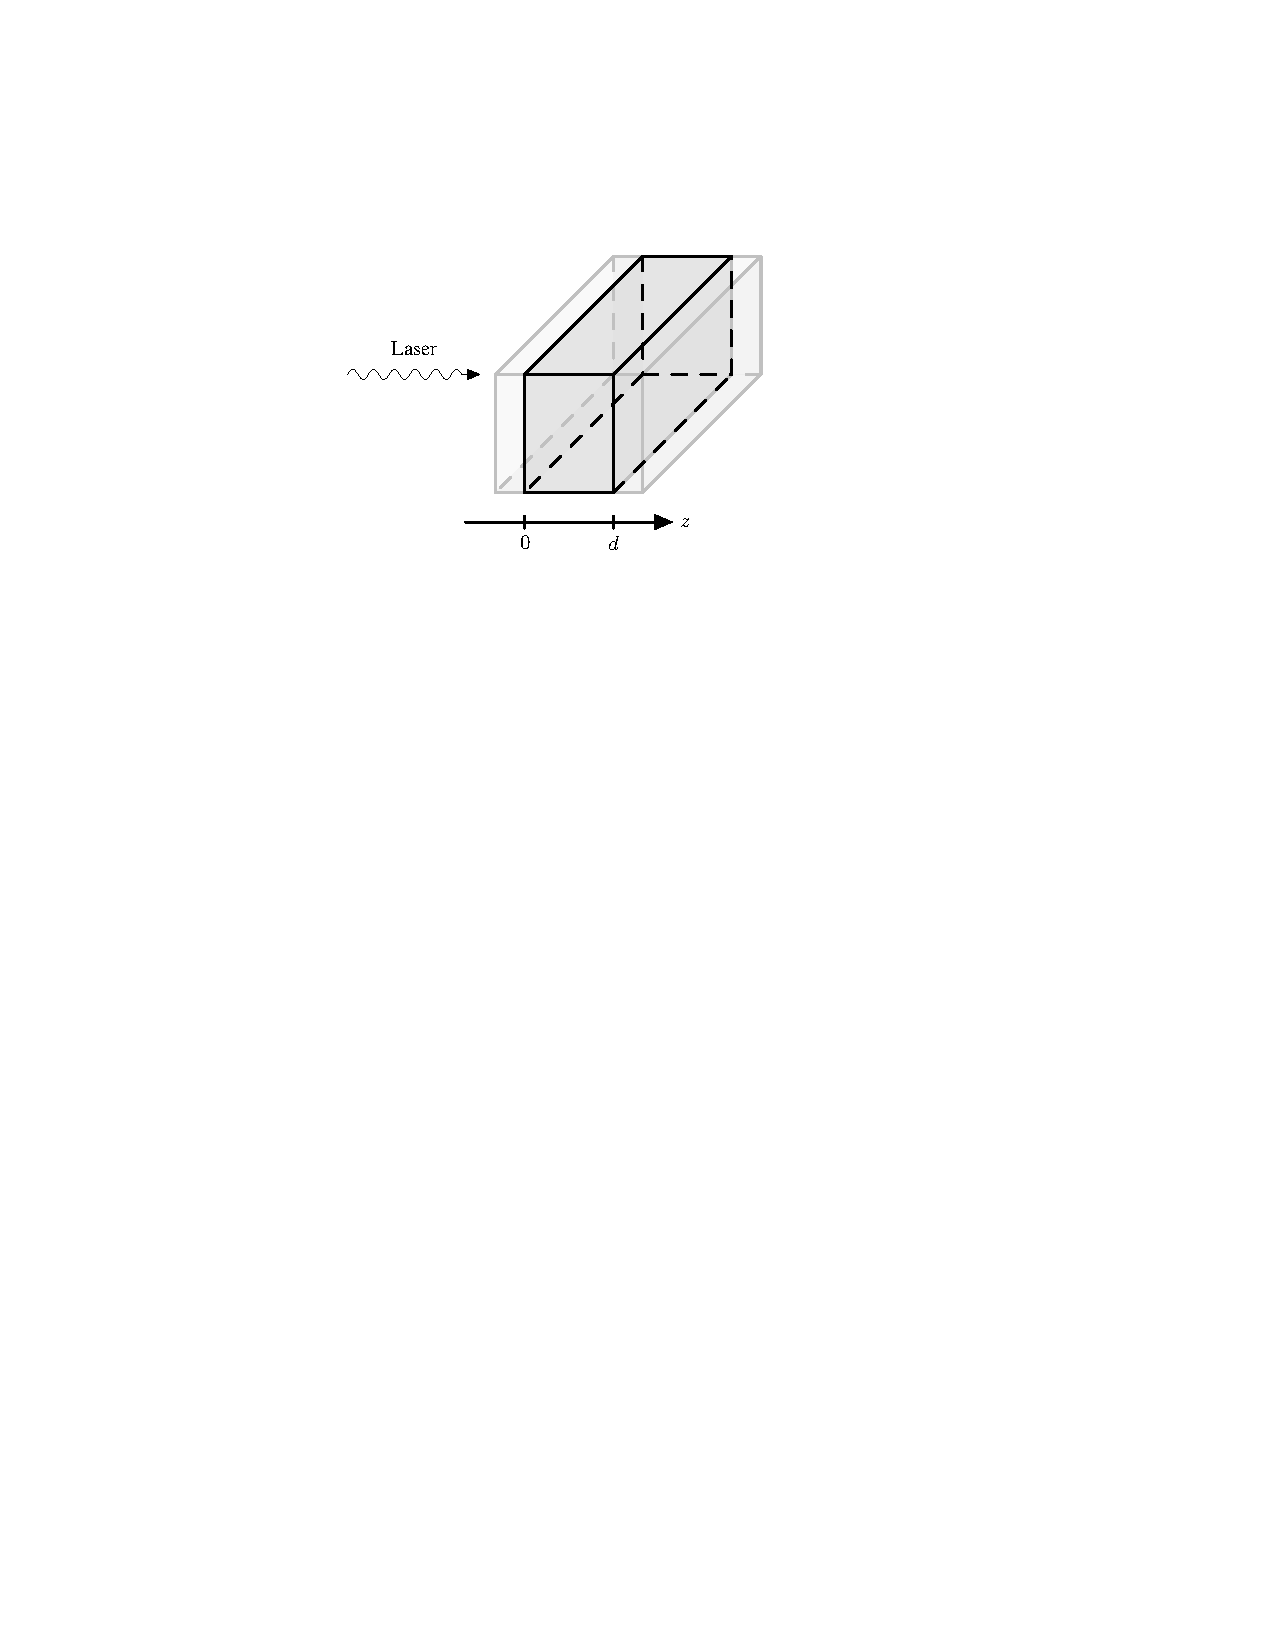
\includegraphics[scale=0.7]{Bilder/Bild1.pdf}
   \caption[Skizze des Aufbaus der Probe]{Skizze des Aufbaus der Probe. Der Halbleiter aus Peroskit liegt zwischen zwei Materialien und wird in der Ebene senkrecht zu $z$ als unendlich ausgedehnt angenommen. Die Bestrahlung mit Laserlicht erfolgt gleichmäßig aus der Richtung $z < 0$.}
   \label{fig:Bild1}
\end{figure}

Hier ist $s(t,z)$ die Ladungsträgerdichte, die durch die Bestrahlung pro Zeiteinheit erzeugt wird, $D$ die Diffusionskonstante, $N_D$ die Dotierungsdichte, $k_1$ bzw.\xspace $k_2$ die Rekombinationskonstanten (Shockley Read Hall Rekombination, bzw.\xspace direkte Rekombination) und $\alpha$ die Absorptionskonstante. Die Konstanten $S_L$ $(z = 0)$ bzw.\xspace $S_R$ $(z = d)$ bestimmen die Rekombinationsraten an den jeweiligen Grenzschichten. \\

In dieser Arbeit sollen folgende Parameter verwendet werden

\begin{table}[H]
   \centering
   \resizebox{0.7\textwidth}{!}{%
      \begin{tabular}{l|l|l|l|l|l|l|l|l}
         Parameter & $d$                  & $D$                               & $K_1$                       & $k_2$                             & $N_D$                             & $S_L$                       & $S_R$                       & $\alpha$                    \\ \hline
         Einheit   & $\left[\mu m\right]$ & $\left[\frac{{cm}^2}{s}\right]$   & $\left[\frac{1}{s}\right]$  & $\left[\frac{{cm}^3}{s}\right]$   & $\left[\frac{1}{{cm}^3}\right]$   & $\left[\frac{cm}{s}\right]$ & $\left[\frac{cm}{s}\right]$ & $\left[\frac{1}{cm}\right]$ \\ \hline
         Wert      & $0.3$                & $0.003$                           & $10^6$                      & $10^{-8}$                         & $10^{15}$                         & $10$                        & $10^5$                      & $10^5$  
      \end{tabular}%
   }
   \caption{Verwendete Parameter}
   \label{tab:Tabelle1}
\end{table}

\textbf{Achtung:} Verwenden Sie in der Simulation durchgehend $\mu m$ und $\mu s$ als Einheit! \\

Die Simulation von \autoref{eq:eq1} wird schrittweise entwickelt. In \autoref{sec:FiniteDifferenzen} wird zunächst die Zeitabhängigkeit vernachlässigt und eine Diskretisierung im Raum der stationären Gleichung mittels finiter Differenzen entwickelt. Der folgende \autoref{sec:ImpliziteEinschrittverfahren} untersucht eine Klasse von numerischen Verfahren zur Lösung von Anfangswertproblemen, die besonders gut für den vorliegenden Fall geeignet sind. Im letzten \autoref{sec:ZeitaufgeloesteSimulation} werden beide Ansätze mithilfe der Linienmethode kombiniert und eine numerische Lösung der Ausgangsgleichung berechnet.

\clearpage

\section{Finite Differenzen der stationären Gleichung} \label{sec:FiniteDifferenzen}

In diesem Teil der Arbeit soll die stationäre Verteilung der Ladungsträger, d.\xspace h.\xspace für den Fall $\partial u/\partial t = 0$, bei kontinuierlicher Bestrahlung modelliert werden. In diesem Fall ist die Gleichung durch

\begin{align}
   \label{eq:eq4}
   D\frac{\partial^2 u}{\partial z^2} - (k_1 + k_2N_D)u - k_2u^2 = -s(z), \quad 0 < z < d
\end{align}

mit Randbedingungen

\begin{align}
   \label{eq:eq5}
   D\frac{\partial u}{\partial z}(0) = S_Lu(0), \quad D\frac{\partial u}{\partial z}(d) = -S_Ru(d)
\end{align}

gegeben. Hier ist $s(z)$ die Ladungsträgerdichte, die pro Zeiteinheit durch die externe Quelle erzeugt wird. \\

Die Gleichung soll näherungsweise mithilfe der Finite Differenzen Methode gelöst werden [4] (benötigte Abschnitte werden auf Moodle bereitgestellt). Dazu wird das Gebiet $z \in [0, d]$ in $M$ gleich große Intervalle der Länge $h$ aufgeteilt und die Knotenpunkte mit $0 = z_0 < z_1 < ... < z_N = d$ bezeichnet. Die genäherte Ladungsdichte an den Stellen $z_i$ wird mit $u_i$ bezeichnet, d.\xspace h.\xspace es soll

\begin{align*}
   u_i \approx u(z_i), \quad i = 0, 1, ..., N
\end{align*}

gelten. Für diese Werte wird ein Gleichungssystem hergeleitet und anschließend numerisch gelöst. Zwischenzeitlich werden Hilfsknoten an den Stellen $z_{-1} = -h$ und $z_{N+1} = d + h$ mit Werten $u_{-1}$ und $u_{N+1}$ verwendet, die jedoch später durch die Randbedingungen eliminiert werden.

\subsection{Lineare stationäre Gleichung}

Im ersten Schritt soll nur der in $u$ lineare Anteil der \autoref{eq:eq4} ohne den quadratischen Term $-k_2u^2$ untersucht werden:

\begin{align}
   \label{eq:eq6}
   D\frac{\partial^2 u}{\partial z^2} - ku = -s(z), \quad 0 < z < d
\end{align}

mit $k = k_1 + k_2N_D$. Die Randbedingungen sind weiterhin durch \autoref{eq:eq5} gegeben. \\

Die Behandlung der stationären Gleichung erfolgt ähnlich zu der in [4, Abschnitt 8.8] beschriebenen Methode. Jedoch werden die Randbedingungen unterschiedlich behandelt. Folgende Aufgaben wurden bearbeitet.

\subsubsection{Methode aus [4, Abschnitt 8.8] für Anwendung auf \autoref{eq:eq6}}

Die beschriebene Methode der finiten Differenzen für Zweipunkt-Randwertprobleme ermöglicht die Lösung von linearen Differenzialgleichungen zweiter Ordnung. Die Grundlage der finiten Differenzen Methode ist das Aufstellen von diskreten Gleichungen durch das Substituieren der Ableitungen mit geeigneten finiten Differenzen. Das Ergebnis ist eine Matrix, mit der in unserem konkreten Beispiel die zeitabhängige Stelle der Ladungsträgerdichte $u_i$ mathematisch beschrieben werden kann. \\

Für die beschriebene Methode sind drei Schritte notwendig:

\begin{enumerate}
   \item Diskretisierung des Bereiches $z \in [0, d]$ in $M$ gleich große Intervalle der Länge $h$ mit $h = \frac{d-0}{N}$.
   \item Diskretisierung der Differenzialgleichung an den Knotenpunkten $u_1, ... , u_{N-1}$ mit den Approximationen der Ableitungen.
   \item Diskretisierung der Randbedingungen und Aufstellen des Gleichungssystems durch die Elimination von $u_{-1}$ und $u_{N+1}$.
\end{enumerate}

\subsubsection{Herleitung der Gleichung für die gesuchten Werte $u_0, ... , u_{N}$}

Approximation der 1. Ableitung:

\begin{align*}
   \frac{\partial u}{\partial z} = \frac{u_{i+1}-u_{i-1}}{2h}
\end{align*}

Approximation der 2. Ableitung:

\begin{align*}
   \frac{\partial^2 u}{\partial z^2} = \frac{u_{i+1}-2\cdot u_i+u_{i-1}}{h^2}
\end{align*}

Durch das Einsetzen der Approximationen der beiden Ableitungen ergeben sich für $u_i$ mit $i=0, ... ,N$ unter der der Festlegung $s_i = s(z_i)$ und $u_i \approx u(z_i)$ folgende Gleichungen:

\begin{align*}
   D\cdot \frac{u_1-2\cdot u_0+\textcolor{blue}{u_{-1}}}{h^2} - k\cdot u_0 &= -s_0 \quad mit \quad i = 0 \\
   D\cdot \frac{u_{i+1}-2\cdot u_i+u_{i-1}}{h^2} - k\cdot u_i &= -s_i \\
   D\cdot \frac{\textcolor{blue}{u_{N+1}}-2\cdot u_N+u_{N-1}}{h^2} - k\cdot u_N &= -s_N \quad mit \quad i = N \\
\end{align*}

Dabei ist $u_i$ die approximierte Ladungsträgerdichte an der Stelle $z_i$ und $s_i$ die Ladungsträgerdichte, die durch die Bestrahlung mit dem Laser an der Stelle $z_i$ auftritt. \\

\subsubsection{Approximation der Ableitungen an den Randbedingungen}

Zunächst werden die ersten Ableitungen an den Randbedingungen (\autoref{eq:eq5}) approximiert durch:

\begin{align*}
   u'(0) \approx \frac{u_1-u_{-1}}{2h}, \quad u'(d) \approx \frac{u_{N+1}-u_{N-1}}{2h}
\end{align*}

Durch das Auflösen nach $u_{-1}$ bzw. $u_{N+1}$ ergibt sich:

\begin{align*}
   u_{-1} = -(u'(0)\cdot 2h) + u_1, \quad u_{N+1} = u'(d)\cdot 2h + u_{N-1}
\end{align*}

Einsetzen an den Knoten $z_0$ und $z_N$ ergibt:

\begin{align*}
   D*\frac{u_1-2u_0-(u'_0\cdot 2h)+u_1}{h^2} - k\cdot u_0 &= -s_0 \quad mit \quad i = 0 \\
   D*\frac{u'_N\cdot 2h+u_{N-1}-2u_N+u_{N-1}}{h^2} - k\cdot u_N &= -s_N \quad mit \quad i = N \\
\end{align*}

Nun können die Randbedingungen aus \autoref{eq:eq5} nach den 1. Ableitungen umgestellt und eingesetzt werden:

\begin{align*}
   u'(0) = \frac{S_L \cdot u_0}{D}, \quad u'(N) = \frac{-S_R \cdot u_N}{D}
\end{align*}

\begin{align*}
   D*\frac{u_1-2u_0-(\frac{S_L \cdot u_0}{D}\cdot 2h)+u_1}{h^2} - k\cdot u_0 &= -s_0 \quad mit \quad i = 0 \\
   D*\frac{\frac{-S_R \cdot u_N}{D}\cdot 2h+u_{N-1}-2u_N+u_{N-1}}{h^2} - k\cdot u_N &= -s_N \quad mit \quad i = N \\
\end{align*}

Die Gleichungen an den Stellen $i=0, i, N$ werden nun vereinfacht bzw. umgeformt:

\begin{align*}
   \frac{D}{h^2}\cdot \left[ \textcolor{green}{2}u_1-\left( \textcolor{green}{2+\frac{s_L\cdot 2h}{D}+\frac{h^2\cdot k}{D}}\right) \cdot u_0\right] &= -s_0 \quad mit \quad i = 0 \\
   \frac{D}{h^2}\cdot \left[ \textcolor{green}{1}u_{i+1}-\left( \textcolor{green}{2+\frac{h^2\cdot k}{D}}\right) \cdot u_i+\textcolor{green}{1}u_{i-1}\right] &= -s_i \\
   \frac{D}{h^2}\cdot \left[ \left( \textcolor{green}{\frac{-s_R\cdot 2h}{D}-2-\frac{h^2\cdot k}{D}}\right) \cdot u_N+\textcolor{green}{2}u_{N-1}\right] &= -s_N \quad mit \quad i = N \\
\end{align*}

\subsubsection{Aufstellen des linearen Gleichungssystems}

Aus den soeben Aufgestellten Gleichungen bzw. den grün eingefärbten Termen wird für die Größen $u_0, ... , u_{N}$ analog zu [4, 8.133] das lineare Gleichungssystem aufgestellt. Dabei soll das Gleichungssystem folgende Form aufweisen:

\begin{align}
   \label{eq:eq7}
   Au = b, \quad u = [u_i], \quad b = [b_i]
\end{align}

Die Gleichungen werden analog zu den Knotenpunkten $z_0, ... , z_N$ geordnet. \\

Für die Koeffizientenmatrix ergibt sich:

\begin{align*}
   A &= \frac{D}{h^2}\cdot
   \begin{bmatrix*}
      \left( 2+\frac{s_L\cdot 2h}{D}+\frac{h^2\cdot k}{D}\right)  & 2 \\
                     1                                            & \left( 2+\frac{h^2\cdot k}{D}\right) & 1 \\
                                                                  & \ddots                               & \ddots & \ddots \\
                                                                                                         &        & 1   & \left( 2+\frac{h^2\cdot k}{D}\right) & 1 \\
                                                                                                         &        &     & 2                                    & \left( \frac{-s_R\cdot 2h}{D}-2-\frac{h^2\cdot k}{D}\right)
   \end{bmatrix*}
   \cdot
   \begin{bmatrix*}
      u_0 \\
      u_1 \\
      \vdots \\
      u_{N-1} \\
      u_N
   \end{bmatrix*}
   \\
   A &= -
   \begin{bmatrix*}
      s_0 \\
      s_1 \\
      \vdots \\
      s_{N-1} \\
      s_N
   \end{bmatrix*}
\end{align*}

\subsubsection{Matlab Routine zum Berechnen der Matrix $A$} \label{sec:test_lin}

Die Routine kann unter dem Dokumentennamen \texttt{fd\_lin\_matrix.m} gefunden werden im beigefügten Ordner.

\subsubsection{Matlab Routine zum Lösen des Gleichungssystems (\autoref{eq:eq7})}

Die Routine kann unter dem Dokumentennamen \texttt{stationär\_lin.m} gefunden werden im beigefügten Ordner.

\subsubsection{Testen der Matlab Routine}

Zum Testen der Routine wird eine Funktion $u(z)$ wie folgt vorgegeben:

\begin{align*}
   u(z) = a \cdot e^{\lambda z}
\end{align*}

Weiterhin werden die Konstanten $d, D, k, a$ und $\lambda$ wie folgt definiert:

\begin{align*}
   d &= 0,3\mu m \\
   D &= 0,003 \frac{cm^2}{s} \\
   k_1 &= 10^6 \frac{1}{s} \\
   k_2 &= 10^{-8} \frac{cm^3}{s} \\
   N_D &= 10^{15} \frac{1}{cm^3} \\
   k &= k_1 + k_2 \cdot N_D \\
   a &= 1 \\
   \lambda &= 1
\end{align*}

Nachfolgend muss die erste und zweite Ableitung der Funktion $u(z)$ ermittelt werden, um eine geeignete rechte Seite $s$ zu berechnen:

\begin{align*}
   u'(z) &= \lambda \cdot a \cdot e^{\lambda z} \\
   u''(z) &= \lambda^2 \cdot a \cdot e^{\lambda z}
\end{align*}

Die rechte Seite $s$ ergibt sich zu:

\begin{align*}
   s = -\left( D \cdot u''(z) - k \cdot u(z) \right)
\end{align*}

Abschließend berechnen sich die Konstanten $S_L$ und $S_R$ zu:

\begin{align*}
   S_L &= D \cdot \lambda \\
   S_R &= -D \cdot \lambda
\end{align*}

Das Matlab Skript mit den Konstanten kann im beigefügten Ordner unter dem Dokumententitel \texttt{konstanten.m} gefunden werden. \\

\autoref{fig:Aufgabe_2_1_7} zeigt die erfolgreiche Testung der Routine Anhand des Vergleiches zwischen der analytischen Lösung und der der Lösung über die implementierte Routine. Anhand des unteren Abschnittes der Grafik kann festgehalten werden, dass die Lösung über die Routine der realen Lösung annähernd entspricht. Der größe Fehler tritt an den Randstellen auf. \\

Weiterhin zeigt \autoref{fig:Aufgabe_2_1_7_b}, dass der absolute Fehler der Methode mit steigender Anzahl an Teilintervallen $N$ abnimmt. Außerdem kann abgelesen werden, dass es sich um ein Verfahren zweiter Ordnung handelt, da der Fehler um zwei Dekaden sinkt, wenn die Anzahl der Teilintervalle um eine Dekade erhöht wird.

\begin{figure}[H]
   \centering
   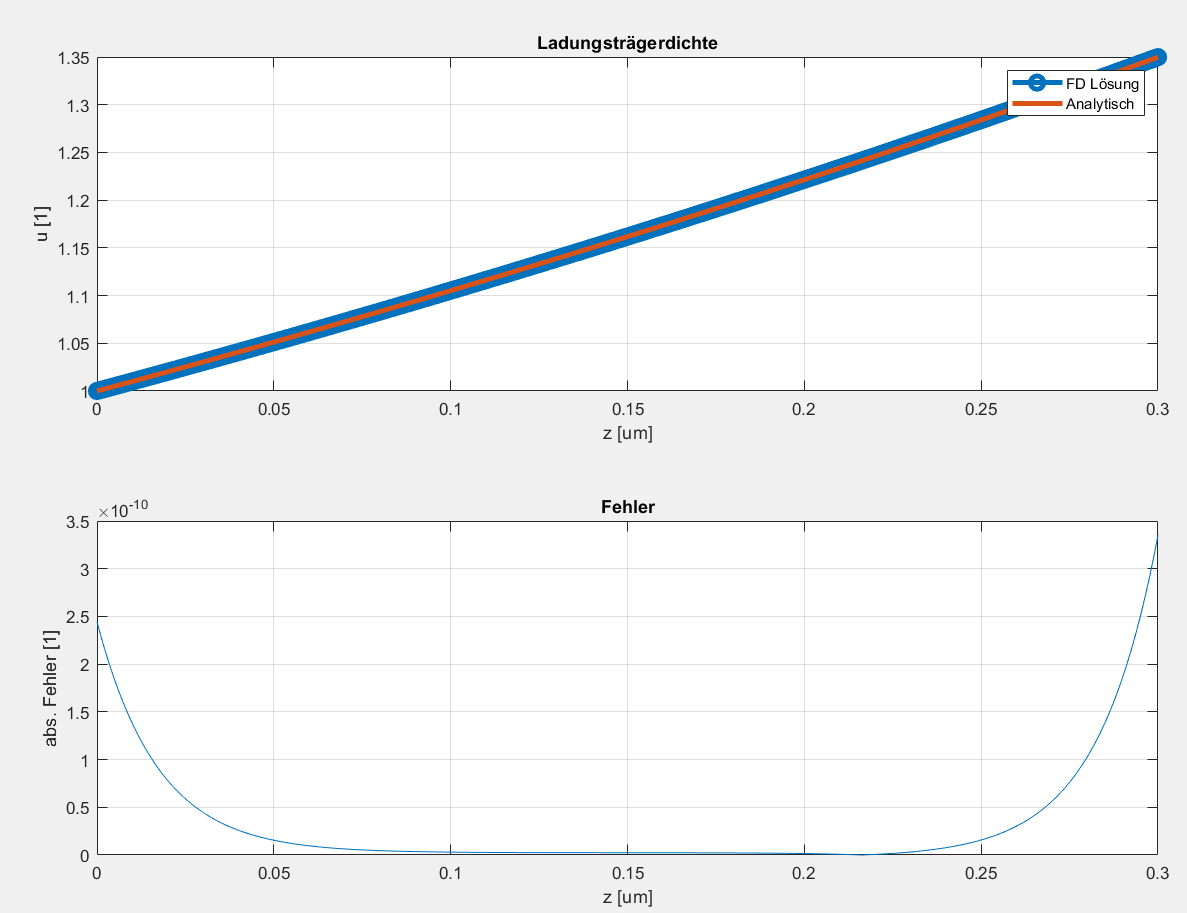
\includegraphics[width=0.82\textwidth]{Bilder/Aufgabe_2_1_7.png}
   \caption[Test der Routine linear stationär]{Vergleich der Analytischen Lösung mit der Lösung über die entwickelte Routine, sowie Darstellung des Fehlers der Lösung mittels der Routine}
   \label{fig:Aufgabe_2_1_7}
\end{figure}

\begin{figure}[H]
   \centering
   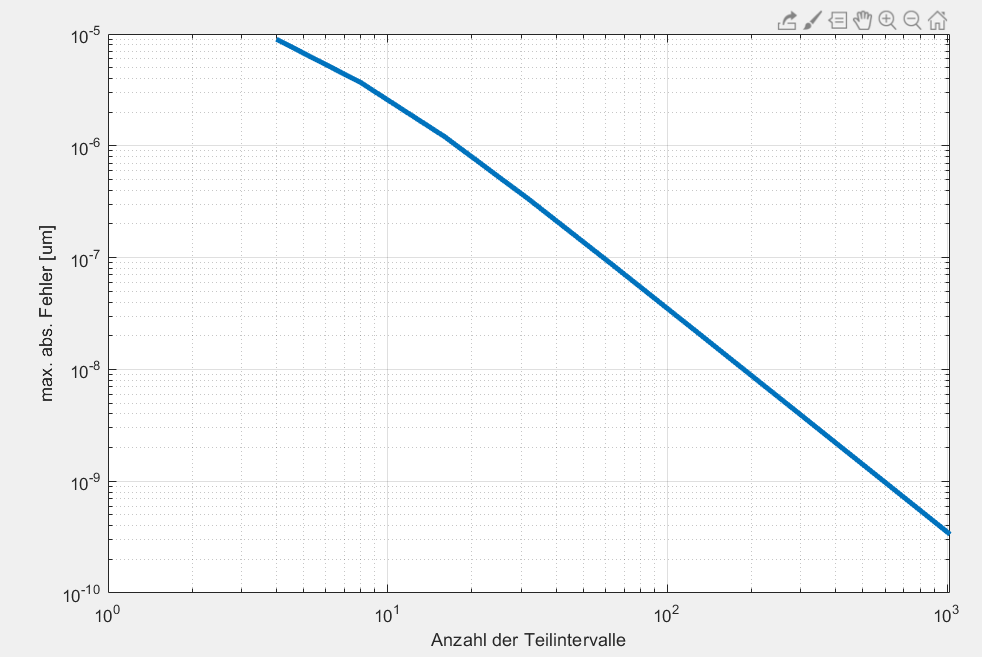
\includegraphics[width=0.7\textwidth]{Bilder/Aufgabe_2_1_7_b.png}
   \caption[Ordnung der Methode linear stationär]{Darstellung zur Ermittlung der Ordnung der Methode}
   \label{fig:Aufgabe_2_1_7_b}
\end{figure}

Die genutzte Matlab Routine zum Testen der Routine kann unter dem Dokumentennamen \texttt{ordnung\_stationär\_lin.m} gefunden werden im beigefügten Ordner.

\subsubsection{Anwendung der Routine auf spezielle Fälle}

In dieser Teilaufgabe soll mit der entwickelten Routine die Lösung für die Fälle

\begin{align*}
   s(z) = S_0 \cdot e^{-\alpha z}, \quad S_0 = 10^2, 10^3, 10^4 \frac{1}{\mu m^3 \mu s}
\end{align*}

berechnet werden. Weiterhin soll ein geeignetes $N$ so bestimmt werden, dass der relative Fehler in $u_i$ maximal 1\textperthousand{} beträgt. \\

Das Ergebnis für die drei Fälle von $S_0$ ist in \autoref{fig:Aufgabe_2_1_8} zu erkennen.

\begin{figure}[H]
   \centering
   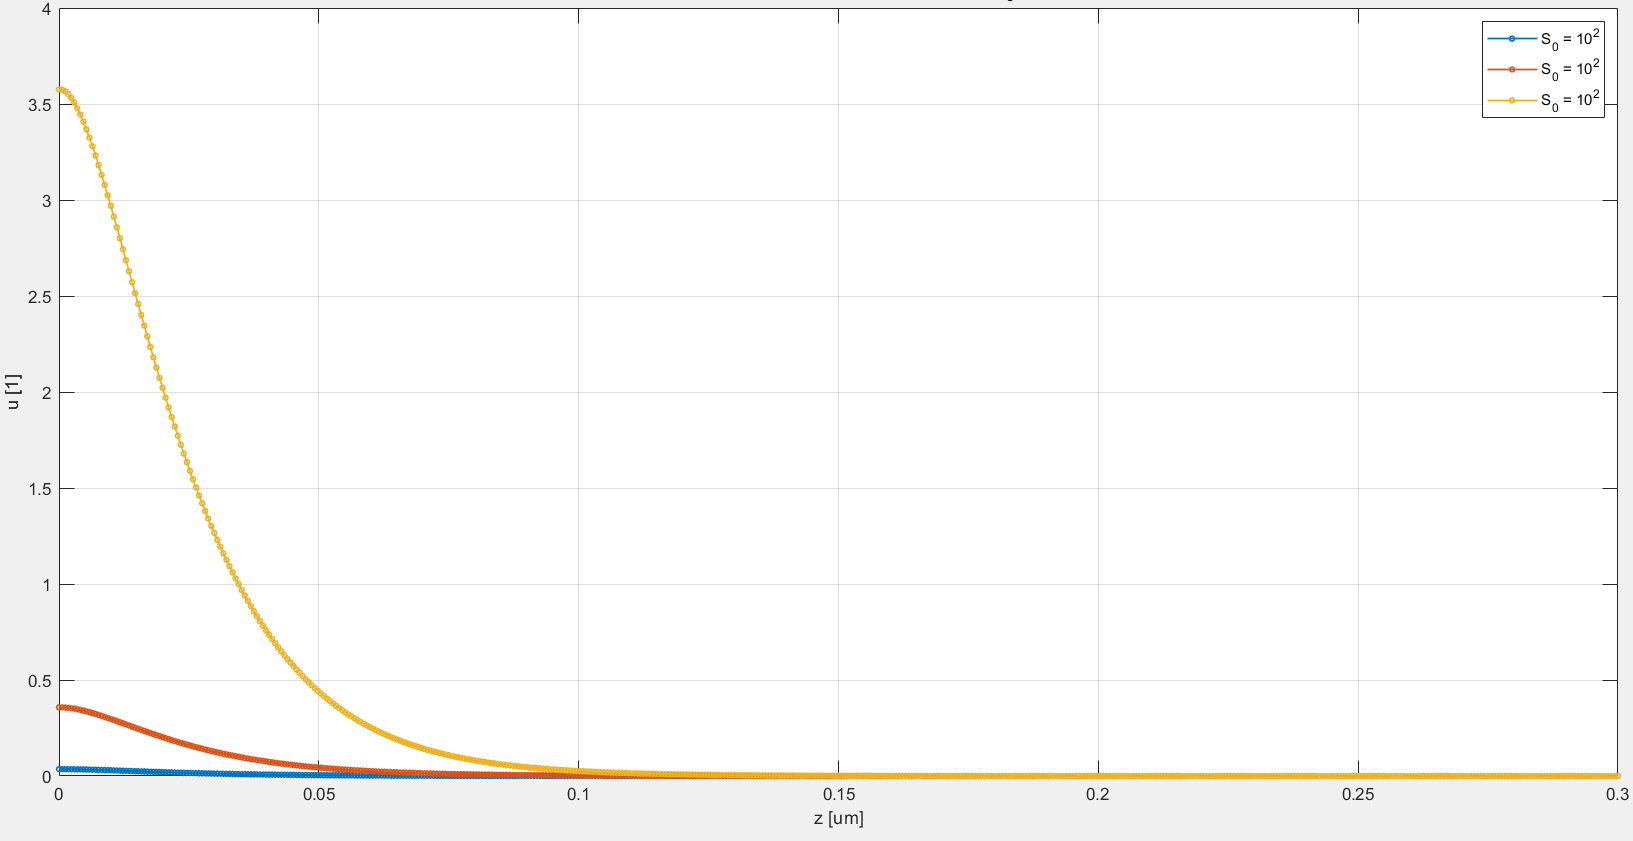
\includegraphics[width=1\textwidth]{Bilder/Aufgabe_2_1_8.png}
   \caption[Lösung von $s(z)$]{Lösung von $s(z)$ für verschiedene $S_0$}
   \label{fig:Aufgabe_2_1_8}
\end{figure}

Um ein geeignetes $N$ zu bestimmen, um den realtiven Fehler zu erreichen, wird das $N$ in einer Schleife iterativ erhöht. Dabei wird der Fehler relativ zum vorherigen $N$ berechnet. Das ergebnis dieser Routine wird in \autoref{fig:Aufgabe_2_1_8_b} dargestellt. \\
Die Routine kann unter dem Dokumentennamen \texttt{exper\_stationär\_lin.m} gefunden werden im beigefügten Ordner. Es kann festgehalten werden, dass das $N$ als 512 gewählt werden muss, um einen relativen Fehler in $u_i$ von maximal 1\textperthousand{} zu erreichen.

\begin{figure}[H]
   \centering
   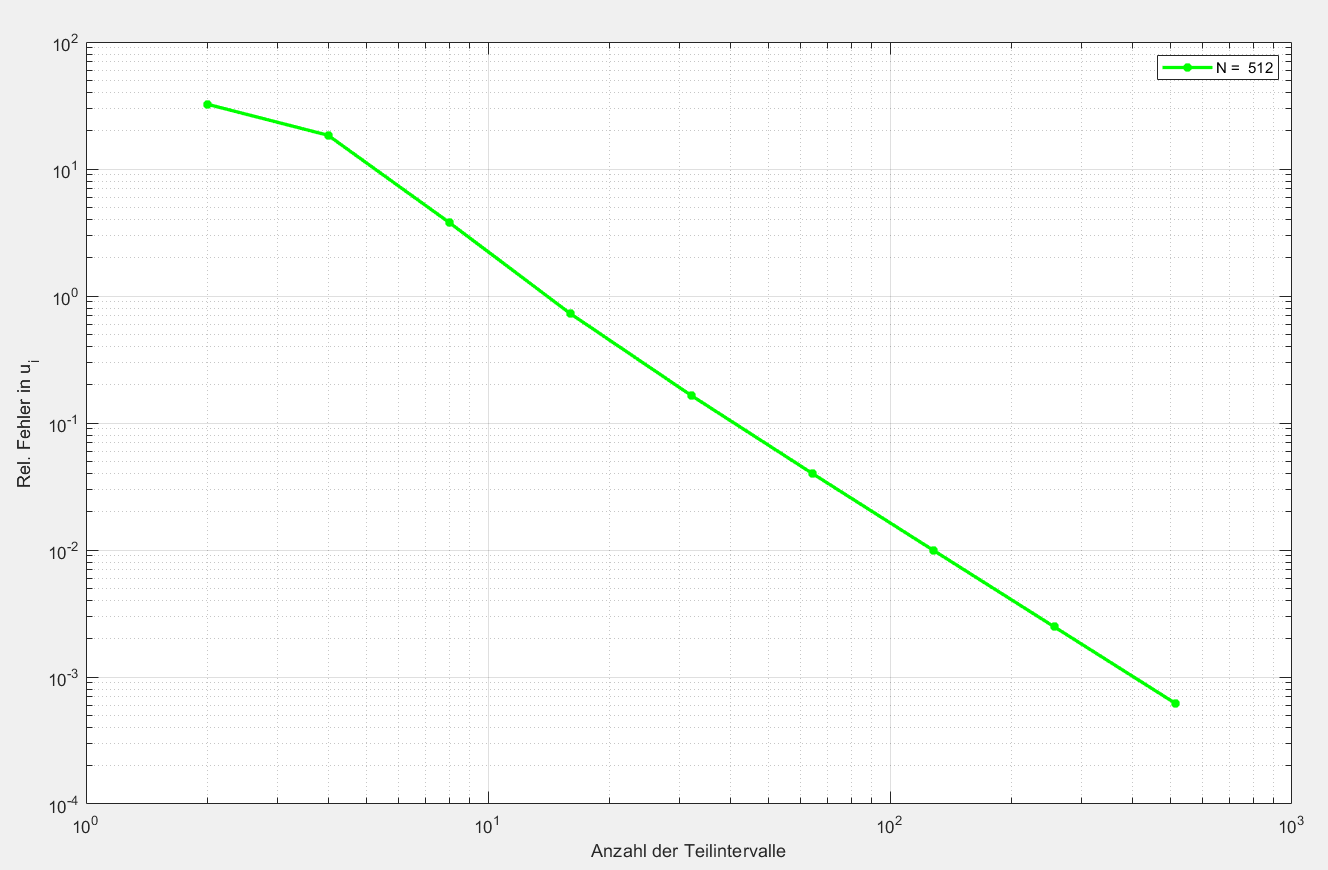
\includegraphics[width=1\textwidth]{Bilder/Aufgabe_2_1_8_b.png}
   \caption[Experimentelle Ermittlung von $N$]{Experimentelle Ermittlung von $N$, so dass der relative Fehler in $u_i$ maximal $10^{-3}$ beträgt}
   \label{fig:Aufgabe_2_1_8_b}
\end{figure}

\subsection{Nichtlineare stationäre Gleichung}

Im zweiten Schritt soll nun die volle nichtlineare Gleichung \autoref{eq:eq4} mit Randbedingung \autoref{eq:eq5} gelöst werden. Analog zum letzten Abschnitt wird ein nichtlineares Gleichungssystem aufgestellt, das mithilfe des Newton-Verfahrens aus der Belegarbeit gelöst werden soll.

\subsubsection{Herleitung der nichtlinearen Gleichungen für die gesuchten Werte $u_0, ... , u_{N}$} \label{sec:nichtlineare_gleichungen}

Die nichtlinearen Gleichungen sollen in der Form

\begin{align}
   \label{eq:eq8}
   F(u) = b
\end{align}

dargestellt werden. Wie auch schon im linearen Fall werden die Randbedingungen berücksichtigt. \\

Zunächst werden wieder die Approximationen der 1. und 2. Ableitung aufgestellt. \\

Approximation der 1. Ableitung:

\begin{align*}
   \frac{\partial u}{\partial z} = \frac{u_{i+1}-u_{i-1}}{2h}
\end{align*}

Approximation der 2. Ableitung:

\begin{align*}
   \frac{\partial^2 u}{\partial z^2} = \frac{u_{i+1}-2\cdot u_i+u_{i-1}}{h^2}
\end{align*}

Durch das Einsetzen der Approximationen der beiden Ableitungen ergeben sich für $u_i$ mit $i=0, ... ,N$ unter der der Festlegung $s_i = s(z_i)$ und $u_i \approx u(z_i)$ folgende Gleichungen:

\begin{align*}
   D\cdot \frac{u_1-2\cdot u_0+\textcolor{blue}{u_{-1}}}{h^2} - k\cdot u_0 -k_2\cdot u_0^2 &= -s_0 \quad mit \quad i = 0 \\
   D\cdot \frac{u_{i+1}-2\cdot u_i+u_{i-1}}{h^2} - k\cdot u_i -k_2\cdot u_0^2 &= -s_i \\
   D\cdot \frac{\textcolor{blue}{u_{N+1}}-2\cdot u_N+u_{N-1}}{h^2} - k\cdot u_N -k_2\cdot u_0^2 &= -s_N \quad mit \quad i = N \\
   mit \quad k = k_1+k_2\cdot N_D
\end{align*}

Anschließend werden die ersten Ableitungen an den Randbedingungen (\autoref{eq:eq5}) approximiert durch:

\begin{align*}
   u'(0) \approx \frac{u_1-u_{-1}}{2h}, \quad u'(d) \approx \frac{u_{N+1}-u_{N-1}}{2h}
\end{align*}

Durch das Auflösen nach $u_{-1}$ bzw. $u_{N+1}$ ergibt sich:

\begin{align*}
   u_{-1} = -(u'(0)\cdot 2h) + u_1, \quad u_{N+1} = u'(d)\cdot 2h + u_{N-1}
\end{align*}

Einsetzen an den Knoten $z_0$ und $z_N$ ergibt:

\begin{align*}
   D*\frac{u_1-2u_0-(u'_0\cdot 2h)+u_1}{h^2} - k\cdot u_0 -k_2\cdot u_0^2 &= -s_0 \quad mit \quad i = 0 \\
   D*\frac{u'_N\cdot 2h+u_{N-1}-2u_N+u_{N-1}}{h^2} - k\cdot u_N -k_2\cdot u_0^2 &= -s_N \quad mit \quad i = N \\
\end{align*}

Nun können die Randbedingungen aus \autoref{eq:eq5} nach den 1. Ableitungen umgestellt und eingesetzt werden:

\begin{align*}
   u'(0) = \frac{S_L \cdot u_0}{D}, \quad u'(N) = \frac{-S_R \cdot u_N}{D}
\end{align*}

\begin{align*}
   D*\frac{u_1-2u_0-(\frac{S_L \cdot u_0}{D}\cdot 2h)+u_1}{h^2} - k\cdot u_0 -k_2\cdot u_0^2 &= -s_0 \quad mit \quad i = 0 \\
   D*\frac{\frac{-S_R \cdot u_N}{D}\cdot 2h+u_{N-1}-2u_N+u_{N-1}}{h^2} - k\cdot u_N -k_2\cdot u_0^2 &= -s_N \quad mit \quad i = N \\
\end{align*}

Die Gleichungen an den Stellen $i=0, i, N$ werden nun vereinfacht bzw. umgeformt:

\begin{align*}
   \frac{D}{h^2}\cdot \left[ \textcolor{green}{2}u_1-\left( \textcolor{green}{\frac{2D+S_L\cdot 2h+h^2k}{D}+\frac{h^2\cdot k_2}{D}\cdot u_0}\right) \cdot u_0\right] &= -s_0 \quad mit \quad i = 0 \\
   \frac{D}{h^2}\cdot \left[ \textcolor{green}{1}u_{i+1}-\left( \textcolor{green}{\frac{2D+h^2k}{D}+\frac{h^2\cdot k_2}{D}\cdot u_i}\right) \cdot u_i+\textcolor{green}{1}u_{i-1}\right] &= -s_i \\
   \frac{D}{h^2}\cdot \left[ \left( \textcolor{green}{\frac{-S_R\cdot 2h-2D-h^2k}{D}-\frac{h^2\cdot k_2}{D}\cdot u_N}\right) \cdot u_N+\textcolor{green}{2}u_{N-1}\right] &= -s_N \quad mit \quad i = N \\
\end{align*}

Die grün makierten Terme werden später für die Jacobi-Matrix benötigt.\\

Abschließend können die Gleichungen in der Form wie in \autoref{eq:eq8} gefordert dargestellt werden:

\begin{align*}
   \begin{bmatrix*}
      F_0 \\
      \vdots \\
      F_i \\
      \vdots \\
      F_{N}
   \end{bmatrix*}
   &=\frac{D}{h^2}\cdot
   \begin{bmatrix*}
      -\left( \frac{2D+S_L\cdot 2h+h^2k}{D}+\frac{h^2\cdot k_2}{D}\cdot u_0\right) \cdot u_0 + 2u_1 \\
      \vdots \\
      u_{i-1}-\left( \frac{2D+h^2k}{D}+\frac{h^2\cdot k_2}{D}\cdot u_i\right) \cdot u_i+u_{i+1} \\
      \vdots \\
      2u_{N-1} + \left( \frac{-S_R\cdot 2h-2D-h^2k}{D}-\frac{h^2\cdot k_2}{D}\cdot u_N\right) \cdot u_N
   \end{bmatrix*}
   \\
   &= -
   \begin{bmatrix*}
      s_0 \\
      \vdots \\
      s_i \\
      \vdots \\
      s_N
   \end{bmatrix*}
\end{align*}

\subsubsection{Matlab Routine zur Berechnung von $F$ der letztem Teilaufgabe}

Die Routine kann unter dem Dokumentennamen \texttt{fd\_nonlin.m} gefunden werden im beigefügten Ordner.

\subsubsection{Berechnung der Jacobi-Matrix $DF$ von $F$ bezüglich $u$}

Allgemein kann die Jacobi-Matrix $DF$ von $F$ bezüglich $u$ wie folgt dargestellt werden:

\begin{align*}
   DF(u) &=
   \begin{bmatrix*}
      \frac{\partial F_0(u)}{\partial u_0} & \hdots & \frac{\partial F_0(u)}{\partial u_i} & \hdots & \frac{\partial F_0(u)}{\partial u_{N}} \\
      \vdots & & \vdots & & \vdots \\
      \frac{\partial F_i(u)}{\partial u_0} & \hdots & \frac{\partial F_i(u)}{\partial u_i} & \hdots & \frac{\partial F_i(u)}{\partial u_{N}} \\
      \vdots & & \vdots & & \vdots \\
      \frac{\partial F_N(u)}{\partial u_0} & \hdots & \frac{\partial F_N(u)}{\partial u_i} & \hdots & \frac{\partial F_N(u)}{\partial u_{N}}
   \end{bmatrix*}
\end{align*}

\clearpage

\begin{landscape}

Mit Hilfe der grün makierten Terme aus \autoref{sec:nichtlineare_gleichungen} kann nun die konkrete Jacobi-Matrix $DF$ aufgestellt werden.

\begin{align*}
   & DF(u) = \frac{D}{h^2}\cdot \\
   &
   \begin{bmatrix*}
      -\left( \frac{2D+S_L\cdot 2h+h^2k}{D}+\frac{h^2\cdot k_2}{D}\cdot u_0\right)  & 2 \\
                     1                                                              & -\left( \frac{2D+h^2k}{D}+\frac{h^2\cdot k_2}{D}\cdot u_i\right)   & 1 \\
                                                                                    & \ddots                                                             & \ddots & \ddots \\
                                                                                                                                                         &        & 1   & -\left( \frac{2D+h^2k}{D}+\frac{h^2\cdot k_2}{D}\cdot u_i\right)   & 1 \\
                                                                                                                                                         &        &     & 2                                                                  & \left( \frac{-S_R\cdot 2h-2D-h^2k}{D}-\frac{h^2\cdot k_2}{D}\cdot u_N\right)
   \end{bmatrix*}
\end{align*}

\end{landscape}

\clearpage

\subsubsection{Matlab Routine zur Berechnung von $DF$ der letztem Teilaufgabe}

Die Routine kann unter dem Dokumentennamen \texttt{fd\_nonlin\_jac.m} gefunden werden im beigefügten Ordner.

\subsubsection{Matlab Routine zur Lösung des Gleichungssystems (\autoref{eq:eq8})}

Über die \textit{Deal}-Funktion von Matlab kann ein Funktionshandle mit den Routinen für $F$ und $DF$ erstellt werden.\\
Als Startwert dient ein Spaltenvekor mit $N+1$ Zeilen die jeweils eine $0$ enthalten.\\
Das Newton-Verfahren zum Lösen Gleichungssystems bekommt den Funktionshandle $f(u)$, den Startwert, die geforderte Toleranz und die maximale anzahl an Schritten übergeben.\\
Die Routine kann unter dem Dokumentennamen \texttt{stationaer\_nonlin.m} gefunden werden im beigefügten Ordner.

\subsubsection{Testen der Matlab Routine}

Zum Testen der Routine wird eine Funktion $u(z)$ wie auch schon in \autoref{sec:test_lin} vorgegeben:

\begin{align*}
   u(z) = a \cdot e^{\lambda z}
\end{align*}

Weiterhin werden die Konstanten $d, D, k, a$ und $\lambda$ wie folgt definiert:

\begin{align*}
   d &= 0,3\mu m \\
   D &= 0,003 \frac{cm^2}{s} \\
   k_1 &= 10^6 \frac{1}{s} \\
   k_2 &= 10^{-8} \frac{cm^3}{s} \\
   N_D &= 10^{15} \frac{1}{cm^3} \\
   k &= k_1 + k_2 \cdot N_D \\
   a &= 1 \\
   \lambda &= 1
\end{align*}

Nachfolgend muss die erste und zweite Ableitung der Funktion $u(z)$ ermittelt werden, um eine geeignete rechte Seite $s$ zu berechnen:

\begin{align*}
   u'(z) &= \lambda \cdot a \cdot e^{\lambda z} \\
   u''(z) &= \lambda^2 \cdot a \cdot e^{\lambda z}
\end{align*}

Die rechte Seite $s$ ergibt sich zu:

\begin{align*}
   s = -\left( D \cdot u''(z) - k \cdot u(z) - k_2 \cdot u(z)^2 \right)
\end{align*}

Abschließend berechnen sich die Konstanten $S_L$ und $S_R$ zu:

\begin{align*}
   S_L &= D \cdot \lambda \\
   S_R &= -D \cdot \lambda
\end{align*}

Das Matlab Skript mit den Konstanten kann im beigefügten Ordner unter dem Dokumententitel \texttt{konstanten.m} gefunden werden. \\

\autoref{fig:Aufgabe_2_2_6} zeigt die erfolgreiche Testung der Routine Anhand des Vergleiches zwischen der analytischen Lösung und der der Lösung über die implementierte Routine. Anhand des unteren Abschnittes der Grafik kann festgehalten werden, dass die Lösung über die Routine der realen Lösung annähernd entspricht. Der größe Fehler tritt an den Randstellen auf. \\

Weiterhin zeigt \autoref{fig:Aufgabe_2_2_6_b}, dass der absolute Fehler der Methode mit steigender Anzahl an Teilintervallen $N$ abnimmt. Außerdem kann abgelesen werden, dass es sich um ein Verfahren zweiter Ordnung handelt, da der Fehler um zwei Dekaden sinkt, wenn die Anzahl der Teilintervalle um eine Dekade erhöht wird.

\begin{figure}[H]
   \centering
   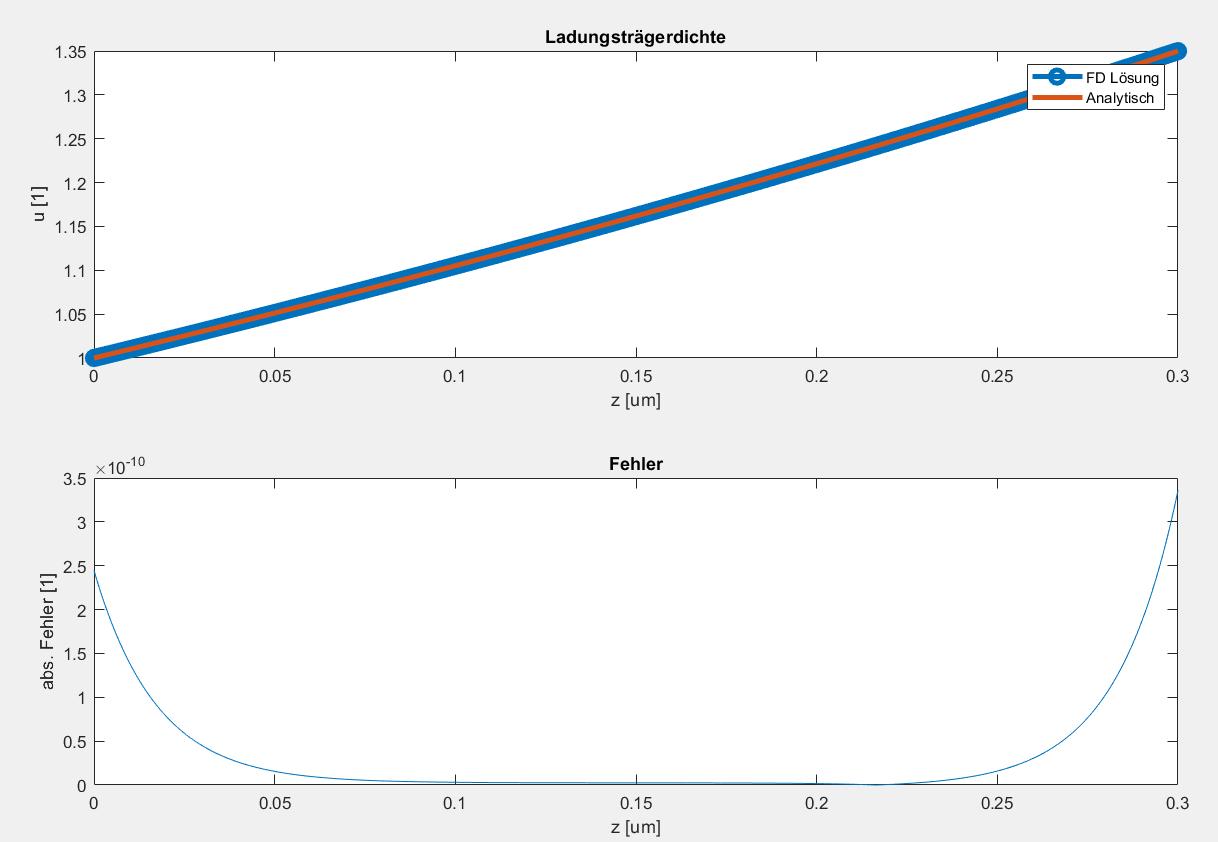
\includegraphics[width=0.82\textwidth]{Bilder/Aufgabe_2_2_6.png}
   \caption[Test der Routine nichtlinear stationär]{Vergleich der Analytischen Lösung mit der Lösung über die entwickelte Routine, sowie Darstellung des Fehlers der Lösung mittels der Routine}
   \label{fig:Aufgabe_2_2_6}
\end{figure}

\begin{figure}[H]
   \centering
   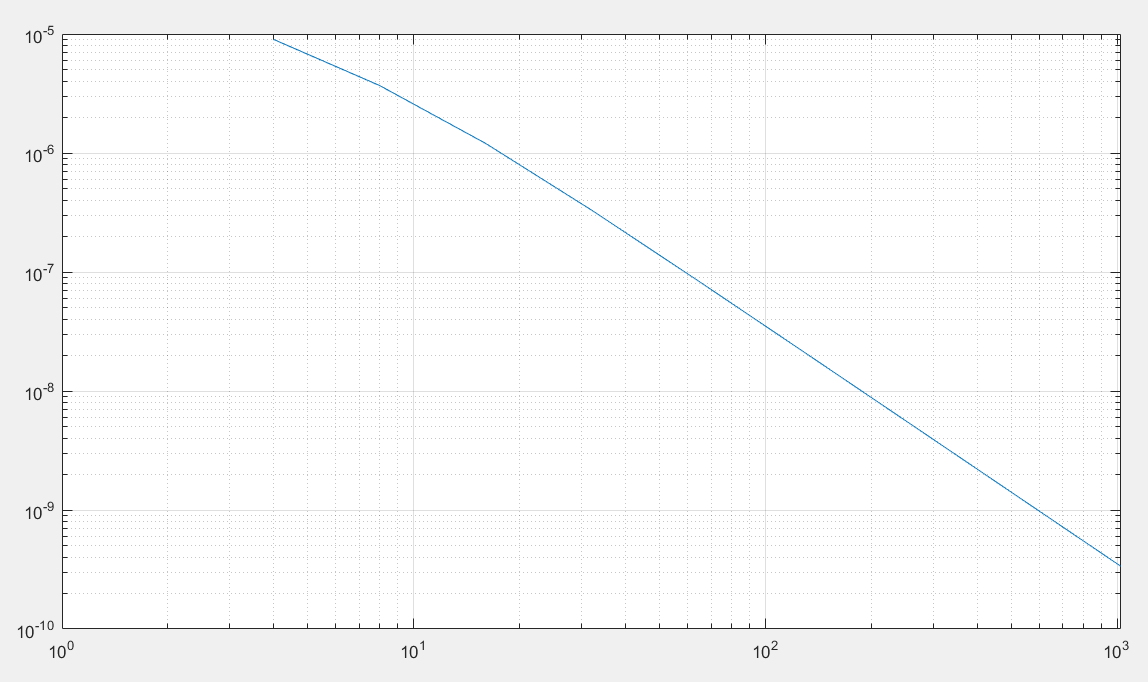
\includegraphics[width=0.7\textwidth]{Bilder/Aufgabe_2_2_6_b.png}
   \caption[Ordnung der Methode nichtlinear stationär]{Darstellung zur Ermittlung der Ordnung der Methode}
   \label{fig:Aufgabe_2_2_6_b}
\end{figure}

Die genutzte Matlab Routine zum Testen der Routine kann unter dem Dokumentennamen \texttt{ordnung\_stationär\_nonlin.m} gefunden werden im beigefügten Ordner.

\subsubsection{Anwendung der Routine auf spezielle Fälle}

In dieser Teilaufgabe soll mit der entwickelten Routine die Lösung für die Fälle

\begin{align*}
   s(z) = S_0 \cdot e^{-\alpha z}, \quad S_0 = 10^2, 10^3, 10^4 \frac{1}{\mu m^3 \mu s}
\end{align*}

berechnet werden. Weiterhin soll ein geeignetes $N$ so bestimmt werden, dass der relative Fehler in $u_i$ maximal 1\textperthousand{} beträgt. \\

Das Ergebnis für die drei Fälle von $S_0$ ist in \autoref{fig:Aufgabe_2_2_7} zu erkennen.

\begin{figure}[H]
   \centering
   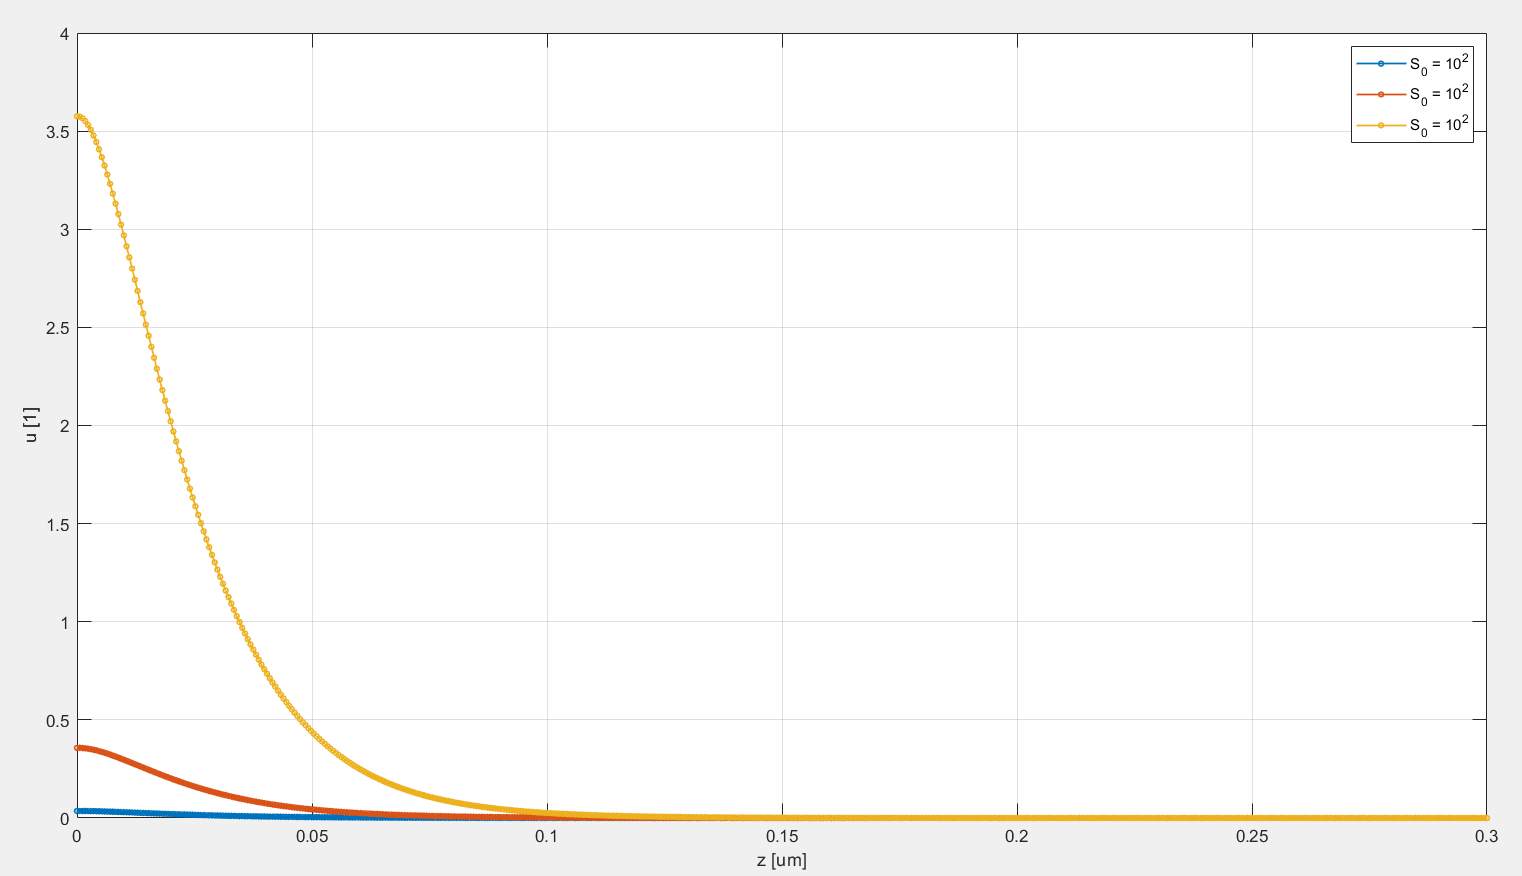
\includegraphics[width=1\textwidth]{Bilder/Aufgabe_2_2_7.png}
   \caption[Lösung von $s(z)$]{Lösung von $s(z)$ für verschiedene $S_0$}
   \label{fig:Aufgabe_2_2_7}
\end{figure}

Um ein geeignetes $N$ zu bestimmen, um den realtiven Fehler zu erreichen, wird das $N$ in einer Schleife iterativ erhöht. Dabei wird der Fehler relativ zum vorherigen $N$ berechnet. Das ergebnis dieser Routine wird in \autoref{fig:Aufgabe_2_2_7_b} dargestellt. \\
Die Routine kann unter dem Dokumentennamen \texttt{exper\_stationär\_nonlin.m} gefunden werden im beigefügten Ordner. Es kann festgehalten werden, dass das $N$ als 512 gewählt werden muss, um einen relativen Fehler in $u_i$ von maximal 1\textperthousand{} zu erreichen.

\begin{figure}[H]
   \centering
   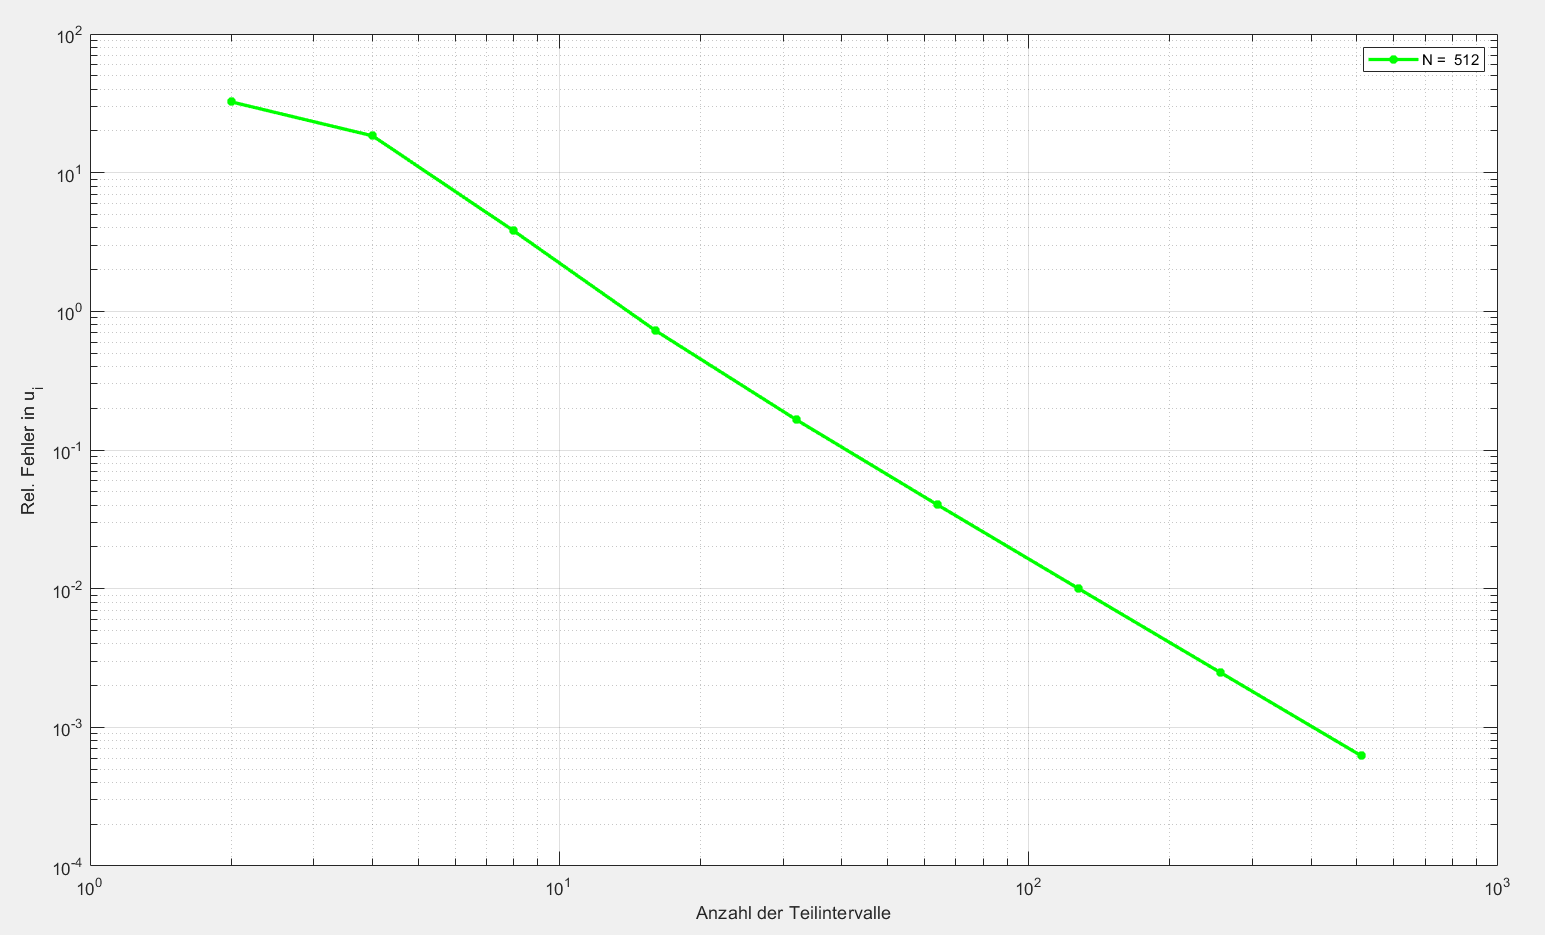
\includegraphics[width=1\textwidth]{Bilder/Aufgabe_2_2_7_b.png}
   \caption[Experimentelle Ermittlung von $N$]{Experimentelle Ermittlung von $N$, so dass der relative Fehler in $u_i$ maximal $10^{-3}$ beträgt}
   \label{fig:Aufgabe_2_2_7_b}
\end{figure}

Beim Vergleich von \autoref{fig:Aufgabe_2_1_8} und \autoref{fig:Aufgabe_2_2_7} kann festgestellt werden, dass die Lösung für alle Fälle gleich scheinen. Auch die experimentelle Bestimmung eines geeigneten $N$ ist gibt sowohl für den linearen, als auch für den nichtlinearen Fall den selben Wert ($N = 512$) zurück.

\clearpage

\section{Implizite Einschrittverfahren} \label{sec:ImpliziteEinschrittverfahren}

In diesem Abschnitt sollen Löser für Systeme von sogenannten steifen Anfangswertproblemen untersucht werden. In \autoref{sec:ZeitaufgeloesteSimulation} wird die partielle Differenzialgleichung \autoref{eq:eq1} mithilfe der finiten Differenzen des letzten Abschnitts näherungsweise als ein System von Anfangswertproblemen formuliert, das sich steif verhält. \\

Steife Systeme treten aber auch in der Modellierung von Reaktionen in der Chemie auf. Als Beispiel soll eine chemische Reaktion dreier Stoffe $A, B, C$ aus [5] dienen:

\begin{align*}
   A \rightarrow B, \quad B +B \rightarrow C + B, \quad B + C \rightarrow A + C
\end{align*}

Die Dynamik der Konzentrationen der einzelnen Komponenten können durch Anfangswertproblem

\begin{align}
   \begin{matrix*}
      A: & y'_1 & = & -0.04y_1   & +10^4y_2y_3                       \\
      B: & y'_2 & = & +0.04y_1   & -10^4y_2y_3  & -3 \cdot 10^7y_2^2 \\
      C: & y'_3 & = &            &              & +3 \cdot 10^7y_2^2
   \end{matrix*}
\end{align}

mit den Anfangswerten

\begin{align}
   y_1(0) = 1, \quad y_2(0) = 0, \quad y_3(0) = 0
\end{align}

modelliert werden. Anhand dieses Systems sollen im folgenden steife Differenzialgleichungen untersucht und ein effizientes numerisches Verfahren entwickelt werden.

\subsection{Entwicklung}

Ein allgemeines System von Anfangswertproblemen für eine Funktion $y : \mathbb{R} \to \mathbb{R} ^k$ kann in der Form

\begin{align}
   \label{eq:eq11}
   y' = f(t,y), \quad t \in [a,b], \quad y(a) = y_a
\end{align}

geschrieben werden. Wie in der Vorlesung wird zur näherungsweisen numerischen Lösung das Intervall $[a,b]$ in $n$ gleich große Teilintervalle der Länge $h$ aufgeteilt mit Knoten $a = t_0 < t_1 < ... < t_n = b$. Der Wert von $y$ wird näherungsweise an diesen Zeitpunkten berechnet:

\begin{align*}
   y^{(i)} \approx y(t_i), \quad i = 0, 1, ..., N.
\end{align*}

Für die Berechnung der Werte $y(i)$ sollen implizite Einschrittverfahren wie in [3, Abschnitt 8.4] verwendet werden. Insbesondere das implizite Euler-Verfahren [3, Gleichung (8.51)]

\begin{align}
   \label{eq:eq12}
   y^{(i+1)} = y^{(i)} + hf(t_{i+1},y^{(i+1)})
\end{align}

und die implizite Trapezregel [3, Gleichung (8.57)]

\begin{align}
   \label{eq:eq13}
   y^{(i+1)} = y^{(i)} + \frac{h}{2}\left[ f(t_{i},y^{(i)}) + f(t_{i+1},y^{(i+1)}) \right]
\end{align}

Im Unterschied zu [3] soll die Lösung der auftretenden nichtlinearen Gleichungssystemen nicht mithilfe der Fixpunktiteration sondern mit dem Newton-Verfahren aus der Belegarbeit näherungsweise bestimmt werden. \\

Dazu wird wie folgt vorgegangen.

\subsubsection{Steife Differenzialgleichungen}

Unter steifen Differenzialgleichungen versteht man Differenzialgleichungen, für welche bestimmte numerische Methoden zum Lösen der Gleichung instabil sind, wenn die Schrittweite nicht extrem klein gewählt wird. Es existieren Differnzialgleichungen, welche Terme besitzen, die zu starken Variationen in der Lösung führen.

\subsubsection{Implizite Verfahren als Nullstellenproblem}

In den Gleichungen des impliziten Euler-Verfahrens und der impliziten Trapezregel (\autoref{eq:eq12} und \autoref{eq:eq13}) wird

\begin{align*}
   y^{(i+1)} = y^{(i)} + z
\end{align*}

gesetzt. Wir erhalten die folgenden Gleichungen für die beiden Verfahren:

\begin{align*}
   Euler: \quad y^{(i)} + z &= y^{(i)} + hf(t_{i+1},y^{(i)} + z) \\
   Trapez: \quad y^{(i)} + z &= y^{(i)} + \frac{h}{2}\left[ f(t_{i},y^{(i)}) + f(t_{i+1},y^{(i)} + z) \right] \\
\end{align*}

Anschließend wird jeweils die Gleichung für $z$ als Nullstellenproblem formuliert:

\begin{align*}
   F_{euler}(z) = 0, \quad F_{trapez}(z) = 0
\end{align*}

Es ergeben sich die folgenden Nullstellenprobleme:

\begin{align*}
   F_{euler}(z) &= z - hf(t_{i+1},y^{(i)} + z) = 0 \\
   F_{trapez}(z) &= z - \frac{h}{2}\left[ f(t_{i},y^{(i)}) + f(t_{i+1},y^{(i)} + z) \right] = 0 \\
\end{align*}

\subsubsection{Jacobi-Matrizen $DF_{euler}$ und $DF_{trapez}$}

Für beide Verfahren soll aus den Gleichungen $F_{euler}(z)$ und $F_{trapez}(z)$ die Jacobi-Matrizen $DF_{euler}$ und $DF_{trapez}$ bestimmt werden in Abhängigkeit von $D_yf$ (der Jacobi-Matrix von $f$ bezüglich $y$).\\

Für das implizite Euler-Verfahren ergibt sich:

\begin{align*}
   DF_{euler}(z) = D \cdot z - D_yf(t_{i+1},y^{(i)} + z)
\end{align*}

Für die implizite Trapezregel ergibt sich:

\begin{align*}
   DF_{trapez}(z) = \frac{h}{2}\left[ D_yf(t_{i},y^{(i)}) + h \cdot D_yf(t_{i+1},y^{(i)} + z) \right] - D \cdot z
\end{align*}

Dabei gilt:

\begin{align*}
   Df =
   \begin{bmatrix*}
      \frac{\partial f_1}{\partial y_1} & \frac{\partial f_1}{\partial y_2} & \cdots & \frac{\partial f_1}{\partial y_n} \\
      \frac{\partial f_2}{\partial y_1} & \frac{\partial f_2}{\partial y_2} & \cdots & \frac{\partial f_2}{\partial y_n} \\
      \vdots & \vdots & \ddots & \vdots \\
      \frac{\partial f_n}{\partial y_1} & \frac{\partial f_n}{\partial y_2} & \cdots & \frac{\partial f_n}{\partial y_n}
   \end{bmatrix*}
\end{align*}

Weiterhin gilt auch:

\begin{align*}
   Df =
   \begin{bmatrix*}
      1 & 0 & \cdots & 0 \\
      0 & 1 & \cdots & 0 \\
      \vdots & \vdots & \ddots & \vdots \\
      0 & \cdots & 0 & 1
   \end{bmatrix*}
\end{align*}

\subsubsection{Matlab Routinenen zur Umsetzung der letzten beiden Teilaufgaben}

Die Routinen können unter den Dokumentennamen \texttt{F\_euler.m} und \texttt{F\_trapez.m} gefunden werden im beigefügten Ordner.

\subsubsection{Löser zu den beiden Verfahren mit Matlab}

Die Löser können unter den Dokumentennamen \texttt{impl\_euler.m} und \texttt{impl\_trapez.m} gefunden werden im beigefügten Ordner.

\subsubsection{Ermittlung der Ordnung der Verfahren}

Die Ermittlung der Ordnung erfolgt anhand des Beispiels

\begin{align*}
   y' = -y
\end{align*}

mit der Anfangsbedingung

\begin{align*}
   y(0) = 1
\end{align*}

auf dem Intervall

\begin{align*}
   t_{span} = [0,1].
\end{align*}

Zunächst wird Differenzialgleichung und deren Ableitung aufgestellt:

\begin{align*}
   f(t,y) = -y \\
   f'(t,y) = -1
\end{align*}

Weiterhin ist die exakte Lösung bekannt:

\begin{align*}
   y = e^{-t}
\end{align*}

In einer Schleife kann nun die Schrittweite iterativ erhöht werden, um die Ordnung der beiden Verfahren grafisch zu ermitteln. \autoref{fig:Aufgabe_3_1_6} und \autoref{fig:Aufgabe_3_1_6_b} zeigen die Ergebnisse. Es ist zu erkennen, dass das implizite Euler-Verfahren eine Ordnung von $1$ hat und die implizite Trapezregel eine Ordnung von $2$.\\
Die Matlab-Scripte können unte den Dokumentennamen \texttt{ordnung\_impl\_euler.m} und \texttt{ordnung\_impl\_trapez.m} gefunden werden im beigefügten Ordner.

\begin{figure}[H]
   \centering
   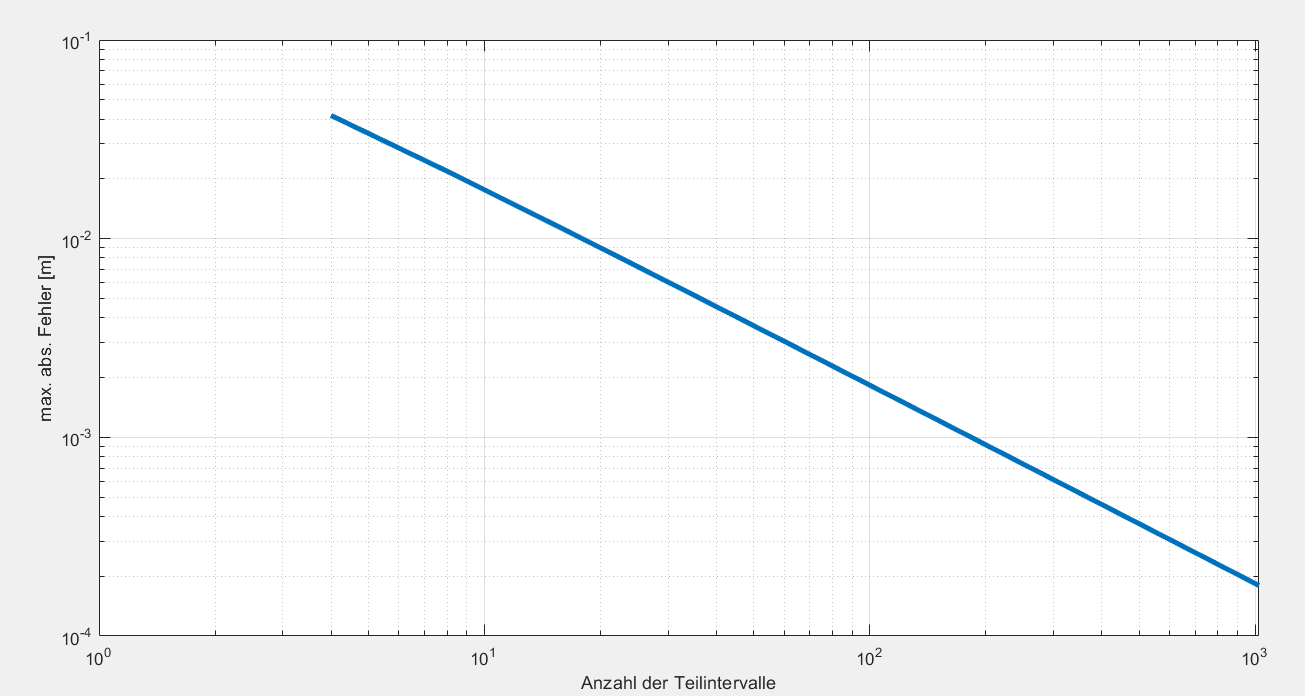
\includegraphics[width=0.9\textwidth]{Bilder/Aufgabe_3_1_6.png}
   \caption[Ordnung impl. Euler-Verfahren]{Grafische Bestimmung der Ordnung des impliziten Euler-Verfahrens}
   \label{fig:Aufgabe_3_1_6}
\end{figure}

\begin{figure}[H]
   \centering
   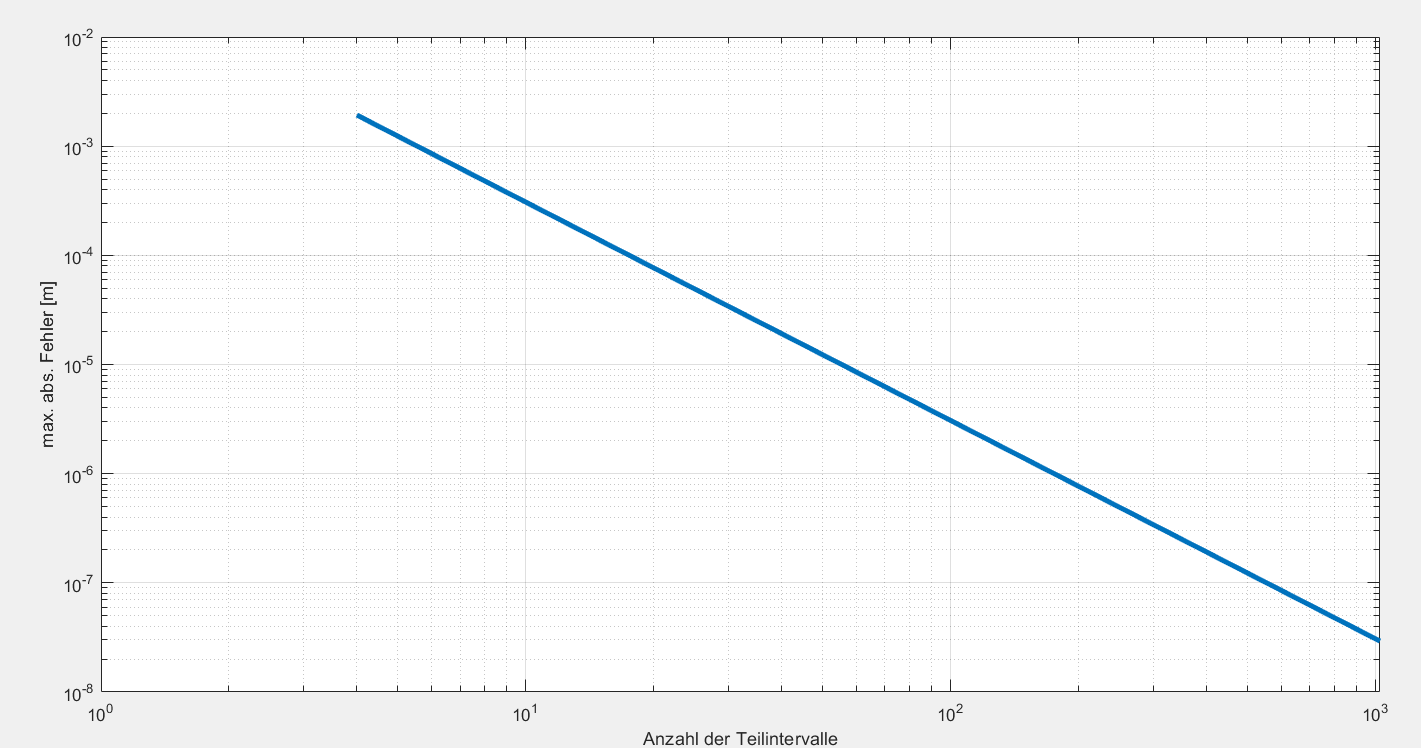
\includegraphics[width=0.9\textwidth]{Bilder/Aufgabe_3_1_6_b.png}
   \caption[Ordnung impl. Trapezregel]{Grafische Bestimmung der Ordnung der impliziten Trapezregel}
   \label{fig:Aufgabe_3_1_6_b}
\end{figure}

\subsubsection{Test der Routine}

Zum Testen der Routine wird eine Lösung und die ersten beiden Ableitungen dieser vorgegeben.

\begin{align*}
   y(t) &= e^{-t} \cdot sin(t) \\
   y'(t) &= e^{-t} \cdot cos(t) - e^{-t} \cdot sin(t) \\
   y''(t) &= -2 \cdot e^{-t} \cdot cos(t)
\end{align*}

Nachfolgend wird eine Differenzialgleichung aufgestellt, die ein System nichtlinearer, zeitabhängiger Anfangswertprobleme beschreibt:

\begin{align*}
   r = y'' + t \cdot y + \omega _0^2 \cdot (y - \frac{1}{6} y^3)
\end{align*}

Nun muss eine rechte Seite ermittelt werden, die für die vorgegebene Lösung passend ist. Dazu wird zunächst ein Spaltenvektor aus der Lösung und deren 1. Ableitung gebildet als Funktionshandle abhängig von $t$ und $z$.

\begin{align*}
   z(t,z) =
   \begin{bmatrix*}
      y(t) \\
      y'(t)
   \end{bmatrix*}
\end{align*}

Nachfolgend wird die Ableitung dieses Vektors bestimmt. Die erste Zeile enthält nun die 1. Ableitung von $y$. Die zweite Zeile enthält die 2. Ableitung von $y$. Durch das Umstellen der Differenzialgleichung $r$ nach $y''$ kann nun wie folgt eingesetzt werden:

\begin{align*}
   f_z(t,z) =
   \begin{bmatrix*}
      y'(t) \\
      r(t) - \left( t \cdot y'(t) + \omega _0^2 \cdot \left( y(t) - \frac{1}{6} \cdot y(t)^3\right) \right)
   \end{bmatrix*}
\end{align*}

Da das Newton-Verfahren auch die Ableitung dieses Vektors benötigt, muss im nächsten Schritt die Jacobi-Matrix berechnet werden.

\begin{align*}
   Df_z(t,z) =
   \begin{bmatrix*}
      0                                            & 1 \\
      -\omega _0 + \omega _0 \cdot 3 \cdot z_1^2  & -t
   \end{bmatrix*}
\end{align*}

Abschließend wird der Startwert ermittelt.

\begin{align*}
   z_0 =
   \begin{bmatrix*}
      y(0) \\
      y'(0)
   \end{bmatrix*}
\end{align*}

Nun können die berechneten Gleichungen als Parameter in der Matlab Routine für die implizite Trapezregel eingesetzt werden. Das Ergebnis ist in \autoref{fig:Aufgabe_3_1_7} dargestellt. \\

Das Matlab-Sckript mit dem Test der Routine kann unter dem Dokumentennamen \texttt{test\_routine.m} gefunden werden im beigefügten Ordner.

\begin{figure}[H]
   \centering
   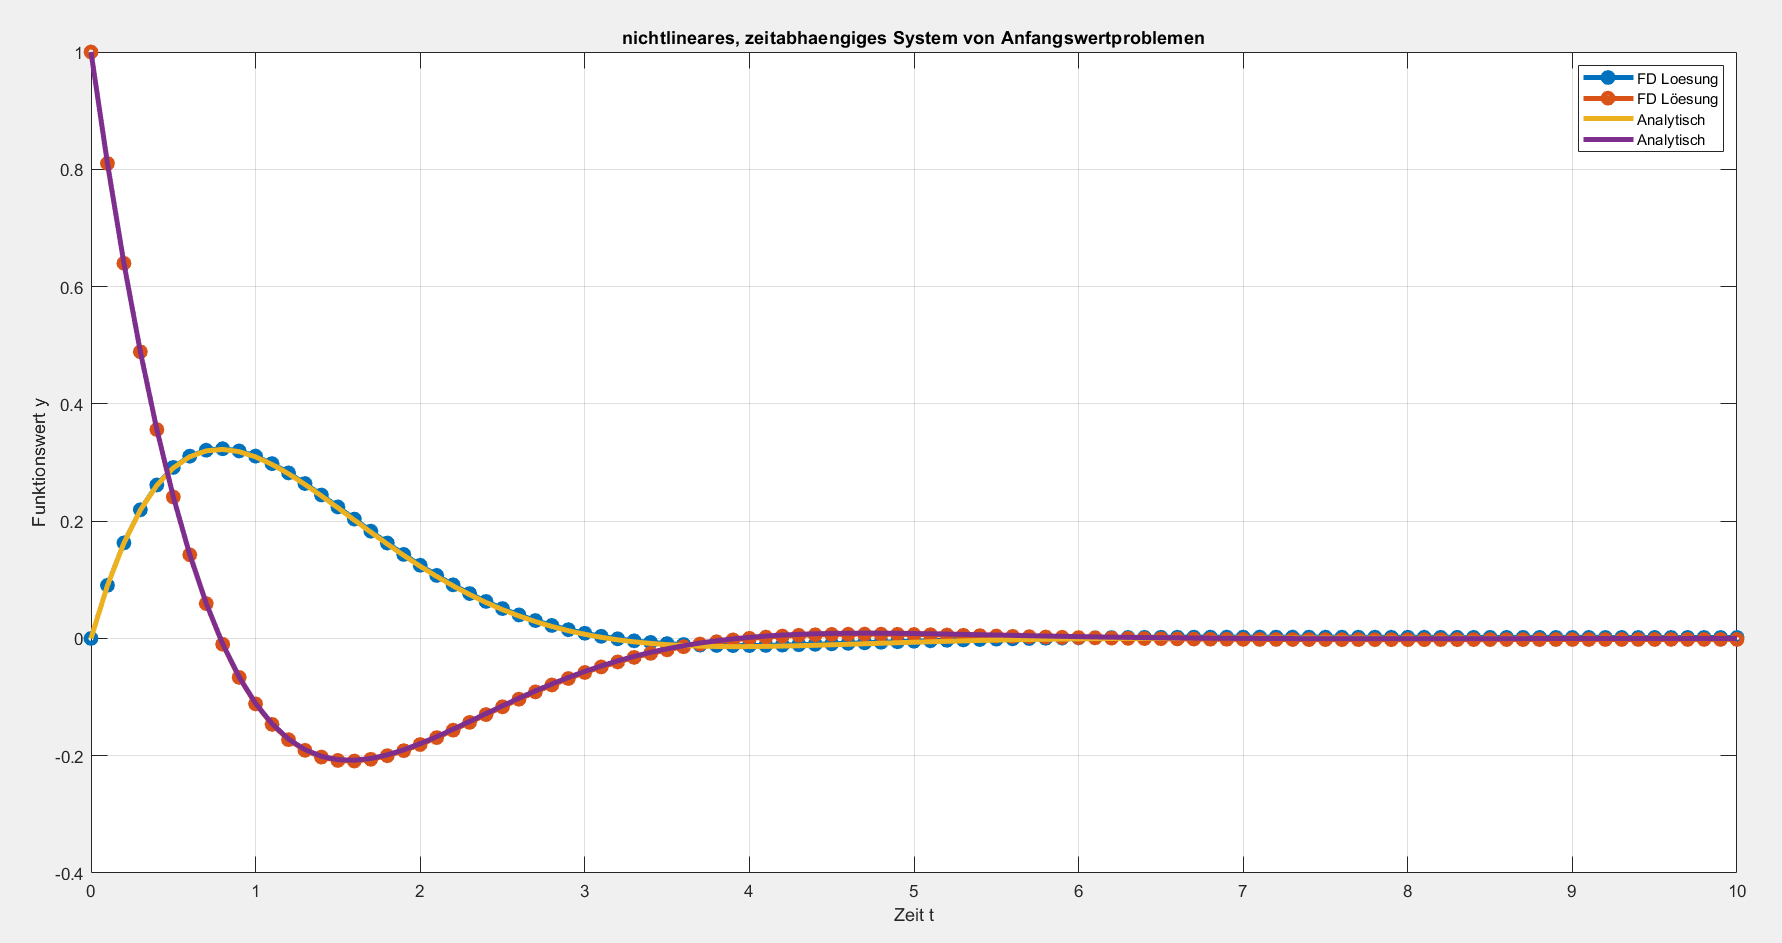
\includegraphics[width=1\textwidth]{Bilder/Aufgabe_3_1_7.png}
   \caption[Test der Routine]{Test der Routine mit einem nichtlinearen, zeitabhängigen System von Anfangswertproblemen}
   \label{fig:Aufgabe_3_1_7}
\end{figure}

\subsection{Anwendung}

\clearpage

\section{Zeitaufgelöste Simulation} \label{sec:ZeitaufgeloesteSimulation}

\clearpage

%---------Quellen---------------------------------
\newpage
\newcount\Quellennummer
\Quellennummer=1

\renewcommand\refname{Literaturverzeichnis}
\addcontentsline{toc}{section}{Literaturverzeichnis}

\begin{thebibliography}{999}
{\setlength{\emergencystretch}{3cm}%

\bibitem[\the\Quellennummer]{HTWgross}
HTW-Logo auf dem Deckblatt\par
\url{https://de.wikipedia.org/wiki/Datei:Logo_HTW_Berlin.svg} \par
 Stand: 17.08.2018 um 14:49 Uhr

\advance\Quellennummer by 1
 
\bibitem[\the\Quellennummer]{HTWklein}
HTW-Logo in der Kopfzeile\par
\url{http://tonkollektiv-htw.de/} \par
 Stand: 17.08.2018 um 14:53 Uhr

\advance\Quellennummer by 1

\bibitem[\the\Quellennummer]{PervoskitSolarCells}
Baloch, Ahmer A. B. \textit{et al:} \glqq Analysis of Photocarrier Dynamics at Interfaces in Pervoskite Solar Cells by Time-Resolved Photoluminescensce\grqq{}, The Journal of Physical Chemistry C, Seiten 26805 - 26815 (2018).

\advance\Quellennummer by 1

\bibitem[\the\Quellennummer]{NumericalAnalysis}
Atkinson, Kendall E. und Han, Weimin: \glqq Elementary Numerical Analysis\grqq{}, J. Wiley \& Sons, Hoboken, NJ (2004).

\advance\Quellennummer by 1

\bibitem[\the\Quellennummer]{StiffDifferentialProblems}
Hairer, Ernst und Wanner, Gerhard: \glqq Solving Ordinary Differential Equations II. Stiff and Differential-Algebraic Problems\grqq{}, Springer, Berlin (1991).

\advance\Quellennummer by 1

}
\end{thebibliography}

\end{document}